\documentclass[a4paper,DIV=12,english]{scrartcl}
\usepackage[utf8]{inputenc}
\usepackage{fancyhdr}
\usepackage{bookmark}
\usepackage{graphicx}
\usepackage{hyperref}
\usepackage{xurl}
\usepackage[sorting=none, style=numeric-comp]{biblatex}
\addbibresource{ref.bib}
\usepackage{csquotes}
\usepackage[dvipsnames]{xcolor}
\usepackage[num]{isodate}
\usepackage{amsthm}
\usepackage{amssymb}
\usepackage{bbm}
\usepackage{amsmath}
\usepackage{tikz}
%\usepackage{pgfplots}
    %\usepgfplotslibrary{fillbetween}
\usepackage{svg}
\usepackage{braket}
\usepackage{caption}
\usepackage{subcaption}
\usepackage{placeins}
%\setlength\parindent{0pt}
\usepackage{wrapfig}
\usepackage{float}

% Fakesection
\newcommand{\fakesection}[1]{%
    \par\refstepcounter{section}                                        % Increase section counter
    \sectionmark{#1}                                                    % Add section mark (header)
    \addcontentsline{toc}{section}{\protect\numberline{\thesection}#1}  % Add section to ToC
    % Add more content here, if needed.
} 

\renewcommand{\footrulewidth}{0.5pt}
\pagestyle{fancy}
\fancyhf{}
\fancyhead[L]{\leftmark}
\fancyhead[R]{}

\fancyfoot[C]{Computational Physics: Band Structure of Lithium using Augmented Plane Waves}
\fancyfoot[R]{\thepage}

\title{Computational Physics: Calculating the Band Structure of Lithium using Augmented Plane Waves}
\author{Stockholm University, Spring Term 2024 \\Max Maschke}
\date{May 29 2024}


\begin{document}
\maketitle


\tableofcontents
\newpage


\newpage
\section{Introduction}
The aim of this report is to introduce and implement the augmented plane wave method for band structure calculation and apply it to Lithium as an example. It is the final report for the Computational Physics course held at Stockholm University in the spring term of 2024.

\section{Electronic States in Periodic Potentials}
Solid state systems such as metallic crystals contain on the order of $10^{23}$ electrons. Their collective behaviour is what determines the bulk properties of the material. A major reason why these properties are at all computationally tractable is symmetry. A crystal (Bravais) lattice in 3D is defined by the fact that there is a set of elementary translation vectors $\{\textbf{a}_1, \textbf{a}_2, \textbf{a}_3\}$ from which every point $\textbf{R}$ or the lattice can be constructed using an integer linear combination:
\begin{equation}
    \textbf{R} = l\textbf{a}_1 + m\textbf{a}_2 + n\textbf{a}_3, \quad l,m,n\in\mathbb{Z}
\end{equation}
This discrete translational symmetry has major implications. Assuming from now on a one-particle picture in which we ignore any interactions of valence and conduction electrons, the electrons feel a potential caused by the ions and core electrons localised at the lattice sites. Because these lattice sites are periodic, the potential is also periodic, i.e.
\begin{equation}
    V(\textbf{r} + \textbf{R}) = V(\textbf{r}).
\end{equation}

\subsection{The Reciprocal Lattice}
The reciprocal lattice is the set of wave vectors $\{\textbf{K}\}$ whose associated plane waves $\text{e}^{i\textbf{k}\textbf{r}}$ are compatible with the periodicity of the real space or direct lattice defined by its elementary translations. That is, it must obey
\begin{equation}
    \textbf{a}_i \cdot \textbf{b}_j = 2\pi \delta_{ij}
\end{equation}
It is obtained via a Fourier transform of the direct lattice and has its own set of elementary lattice vectors
\begin{equation}
    \textbf{b}_1 = \frac{2\pi}{V} \textbf{a}_2 \times \textbf{a}_3 \quad \text{and cyclic.}
\end{equation}
Here, $V=\textbf{a}_1 \cdot (\textbf{a}_2 \times \textbf{a}_3)$ is the volume of the unit cell of the direct lattice~\cite{theoFestkörper}.

\subsection{Bloch's Theorem}
Due to the periodicity of the potential, it has a Fourier representation
\begin{equation}
    V(\textbf{r}) = \sum_\textbf{K} V_\textbf{K} \text{e}^{i\textbf{K}\textbf{r}} 
\end{equation}
where the sum runs over the reciprocal lattice.

Similarly, but distinctly, we can represent a given single particle wave function $\psi$ as 
\begin{equation}
    \psi(\textbf{r}) = \sum_\textbf{q} c_\textbf{q} \text{e}^{i\textbf{q}\textbf{r}} 
\end{equation}
where the sum runs over all wave vectors compatible with the boundary conditions. For infinite system, this becomes an integral over all of $\mathbb{R}^3$.

Plugging both into the single particle Schrödinger equation, one can show without great difficulty~\cite{Thijssen2007cp} that with $\textbf{k}=\textbf{q} + \textbf{K}$ the eigenstates have the form 
\begin{equation}
    \psi_\textbf{k}(\textbf{r}) = \text{e}^{i\textbf{k}\textbf{r}} u_\textbf{k}(\textbf{r})
\end{equation}
where $u$ is a function that shares the periodicity of the lattice. This is known as Bloch's theorem. Its power lies in the fact that it is sufficient to limit ones' analysis to the momenta inside a unit cell of the reciprocal lattice to describe the states of the whole direct lattice. Usually, one chooses the first Wigner-Seitz cell of the reciprocal cell for this purpose, which is also known as the first Brillouin zone.

\subsection{Tight Binding vs Quasi-Free Electrons}
The question of what the dispersion $E(\textbf{k})$\footnote{$E(\textbf{k})$ is usually not a unique function, to uniquely describe an electronic state, the entire tuple ($E$, \textbf{k}) (and possibly $\sigma$) must be specified.} of the lattice electrons looks like is at the core of band structure analysis and its answer can give fundamental insights into a material's properties, such as whether it conducts electric currents.

There are two very simple approaches to this question that have since been built upon, which make qualitatively very different assumptions.

A tight binding approach assumes the valence electrons are localised at the lattice sites\footnote{It is not necessarily obvious what these localised states should look like. The Wannier basis is a popular choice.} but can transition between them with some amplitude $t$. For a simple 1D chain with lattice constant $a$, such a model might read 
\begin{equation}
    \mathcal{H} = \sum_{i, \sigma} t \left( c^\dagger_{i,\sigma} c_{i+1,\sigma} + c^\dagger_{i+1,\sigma} c_{i,\sigma}\right).
\end{equation}
This can be directly solved via a Fourier transform and the dispersion is~\cite{theoFestkörper}
\begin{equation}
    \varepsilon_k = -2t\cos(ka) + \text{const}.
\end{equation}
Cosine-shaped bands are typical for tight binding calculations.

The other approach is to start from free electrons, which have a quadratic dispersion $E\sim k^2$ and whose wave functions are plane waves, and apply perturbation theory. The advantage of this approach is that it is able to produce gaps between energy bands.

However, both approaches are incredibly basic and only rarely accurately describe the true band structure of real crystals. They are however instructive as starting points from which to understand more sophisticated methods.


\section{Augmented Plane Waves}
We have recalled that assembling electronic states from neither plane waves nor atomic wave functions is incredibly successful on its own. One might then reasonably ask whether any improvements are to be gained by combining both ideas somehow. In a seminal paper~\cite{SLATER196435}, Slater proposed just this in an approach which is now known as augmented plane waves (APW). The idea is to compose the state from the atomic functions close to the ions and from plane waves further out.

\subsection{The Muffin Tin Approximation and Muffin Tin Orbitals}
By choosing a radius $R$ around the ions in which we assume the electrons to be comparatively strongly bound and thus described by a superposition of atomic states, we're performing what's known as the muffin tin approximation. These atomic states are not eigenstates but are solutions at a prescribed energy $E$. For systems with one valence electron, they may be obtained by first finding a reasonable single particle potential and then shooting the solutions from $r=0$ to $R$ using an iterative solver such as the ever-popular RK4. Outside the radius $R$, we assume the potential to vanish, which is where this approximation gets its curious name, cf.\ figure~\ref{fig:mtinapprox}.

\begin{figure}
    \centering 
    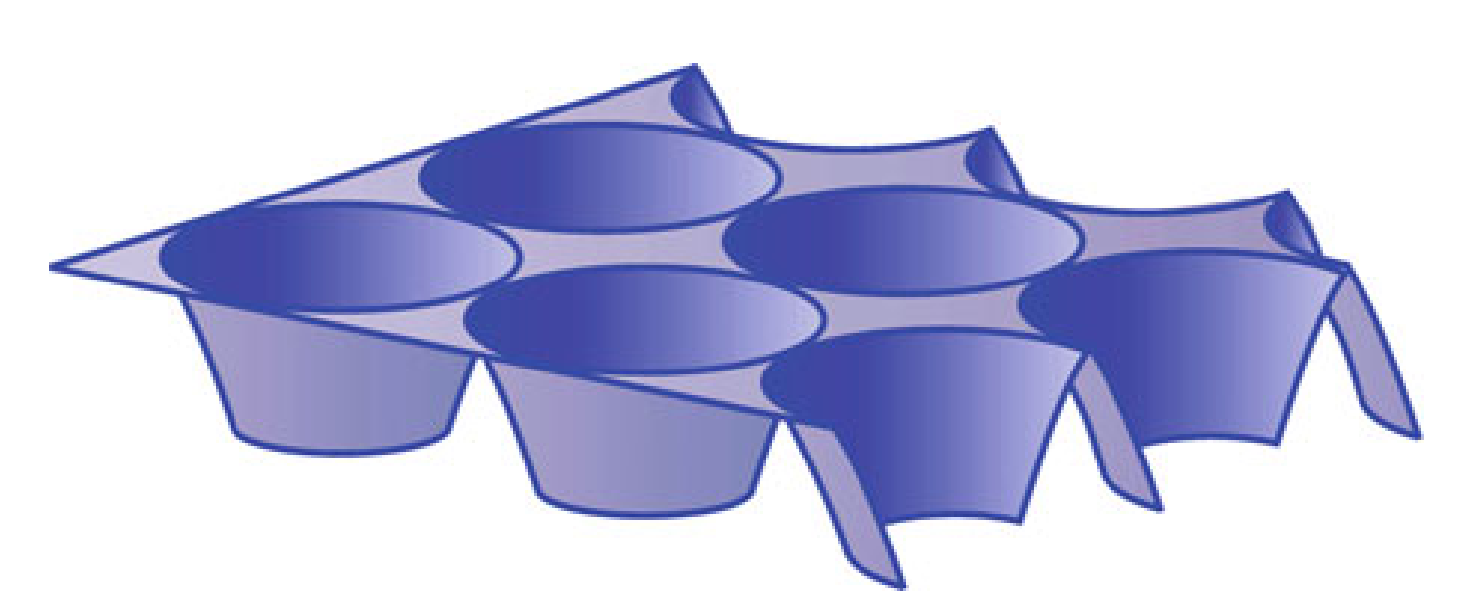
\includegraphics[width=0.65\textwidth]{./fig/mtin.png}
    \caption{Muffin tin approximation, illustration~\cite{Böer2019}. The potential is set to zero outside the spheres with radius $R$.}
    \label{fig:mtinapprox}
\end{figure}

The potential $V(r)$ is in our case obtained using the DFT code previously produced for this course, which was based on the local density approximation.

We then iterate the equation for the radial function $P_{l,E}(r)$ for a given energy $E$ and $l$
\begin{equation}
    \partial_r^2 P_{l,E}(r) = \left(\frac{l(l+1)}{r^2} + 2V(r) - 2E\right)P_{l,E}(r)
\end{equation}
using the initial conditions
\begin{equation}
    P_{l,E}(r) = 0, \quad \partial_r P_{l,E}(r)|_{r=0} = r^l.
\end{equation}
Note that $P_{l,E}(r)/r = R_{l,E}(r)$ is the radial wave function.

\subsection{Constructing the Augmented Basis}
The $R_{l,E}$ depend on the choice of $E=k^2/2$ for a given plane wave $\text{e}^{i\textbf{k}\textbf{r}}$, while the latter also depends on the orientation of $\textbf{k}$. Matching them at the muffin tin boundaries is thus slightly non-trivial and results in a discontinuous derivative with functions of the form~\cite{Thijssen2007cp} 
\begin{equation}
    \psi^{\text{APW}}_\textbf{k} (\textbf{r}) = 
    \begin{cases}
        4\pi \sum_{lm}i^l j_l(kR)\frac{R_{l,k^2/2}(r)}{R_{l,k^2/2}(R)} Y^{l*}_m (\theta_k, \varphi_k) Y^{l}_m (\theta_r, \varphi_r), & r \leq R \\
        \text{e}^{i\textbf{k}\textbf{r}}, & r > R
    \end{cases} 
\end{equation}
where $j_l$ are the spherical Bessel functions and the $Y^l_m$ the spherical harmonics. The sum does in principle run over all allowed values of $l$ and $m$ but is in practice truncated to some $l_\text{max}$ which we chose as 6.

\subsection{Solving for the Electronic States}
We want to find Bloch states for the valence electrons of the form 
\begin{equation}
    \psi_\textbf{k}(\textbf{r}) = \sum_\textbf{K} c_\textbf{K} \psi^{\text{APW}}_{\textbf{k} + \textbf{K}}(\textbf{r}),
\end{equation}
where the sum over all reciprocal lattice vectors is in practice truncated beyond some cut-off $K_\text{max} = |\textbf{K}_\text{max}|$.
The coefficients $\textbf{c}$ minimise the energy mismatch inside and outside the muffin tins. Finding them is rather complicated as they are given by the solutions of a matrix equation 
\begin{equation}\label{eq:evalprob}
    (H_E - EI)\textbf{c} = 0
\end{equation}
where the matrix $H_E$ depends on energy, which prevents us from using the usual tools of linear algebra for solving eigenvalue problems. The matrix elements are given by~\cite{Thijssen2007cp}
\begin{align}
    H_{E,ij} &= \braket{\textbf{k}+\textbf{K}_i|H_E|\textbf{k}+\textbf{K}_j} = -E\,A_{ij} + B_{ij} + \sum_l C_{ijl} \frac{R'_{l, E}(R)}{R_{l, E}(R)} \\
    A_{ij} &= -\frac{4\pi R^2}{V} \frac{j_1\left( \left|\textbf{K}_i - \textbf{K}_j\right|\cdot R \right)}{\left|\textbf{K}_i - \textbf{K}_j\right|} + \delta_{ij} \\
    B_{ij} &= \frac{1}{2}A_{ij}\, \left(\textbf{k}+\textbf{K}_i\right) \cdot \left(\textbf{k}+\textbf{K}_j\right) \\
    C_{ijl} &= (2l+1)\frac{2\pi R^2}{V} P_l\left(\frac{\left(\textbf{k}+\textbf{K}_i\right) \cdot \left(\textbf{k}+\textbf{K}_j\right)}{\left|\textbf{k}+\textbf{K}_i\right| \left|\textbf{k}+\textbf{K}_j\right|}\right) j_l(\left|\textbf{k}+\textbf{K}_i\right|R) j_l(\left|\textbf{k}+\textbf{K}_j\right|R).
\end{align}
Note that here, $P_l$ denotes the Legendre polynomials and not a radial function.

Given the unfavourable structure of~\eqref{eq:evalprob}, one is forced to find the generalised eigenvalues $E$ which give the dispersion by scanning a dense discrete interval of energies and calculating the determinant $\det\left(H_E - EI\right)$.

\section{Solid State Lithium}
\begin{figure}
    \centering 
    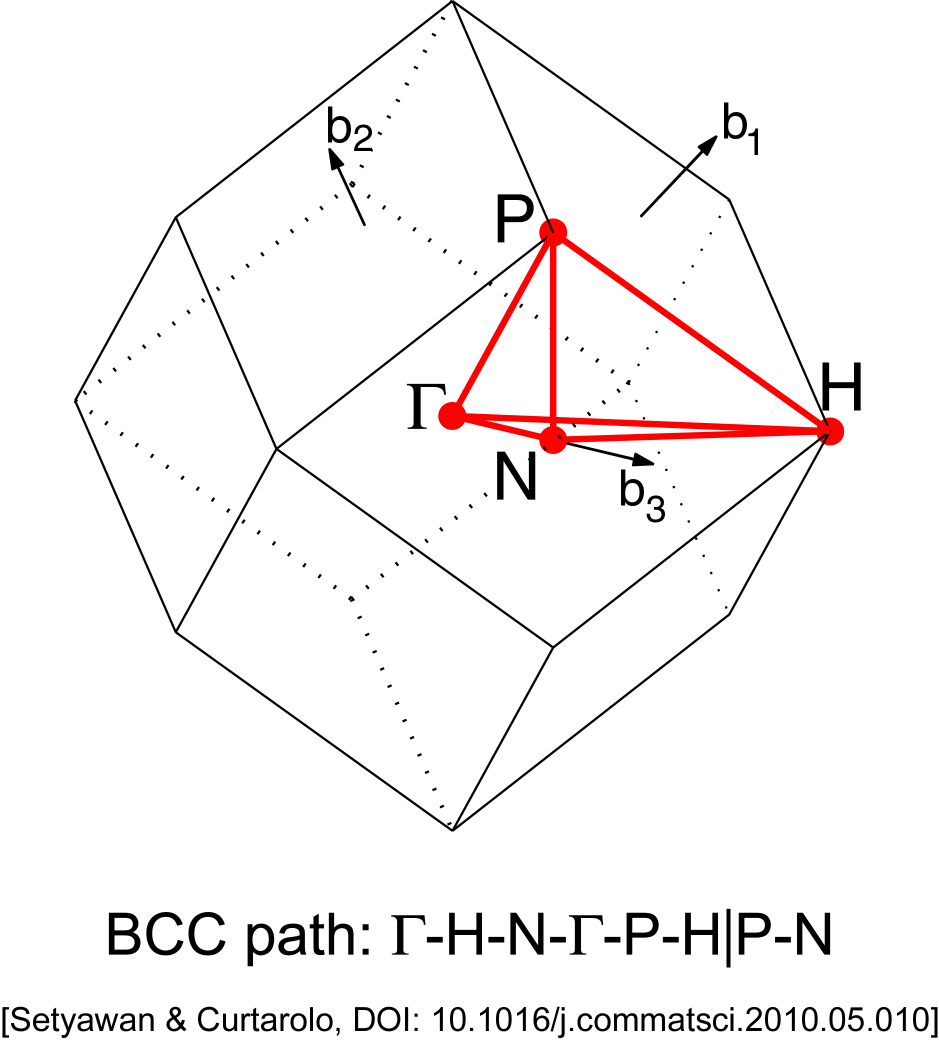
\includegraphics[width=0.55\textwidth]{./fig/bcc_bz.png}
    \caption{Brillouin zone for a BCC lattice. The indicated path follows high symmetry directions of the BZ. Image credit indicated.}
    \label{fig:bcc_bz}
\end{figure}
Lithium is the third element of the periodic table, consisting of a triply charged nucleus and three electrons. As an alkaline metal, it is soft and highly reactive. Nevertheless, it is crystalline in the bulk, growing body centric cubic (BCC) lattices with lattice constant $a=350.0\,\text{pm}=6.632\,a_0$~\cite{wikiLithium}. The Brillouin zone (BZ) of the BCC lattice is shown in figure~\ref{fig:bcc_bz}. Band structures are usually plotted against high-symmetry paths in the BZ, such a path is indicated in the figure for the BCC case.

The electronic structure of Lithium atoms is $1s^22s^1$ in the orbital picture. In this analysis, we only consider the valence electron to be responsible for Lithiums band structure.

\FloatBarrier
\section{Numerical Implementation}
We implement the APW method in a \texttt{C++} class \texttt{apw.h}. The algorithm can be summarised as follows:
\begin{enumerate}
    \item The core potential is obtained by solving the self-consistency equations for the ionic problem as described in the last report using the \texttt{atom.h} class. We use a convergence tolerance for the total energy of $5\cdot 10^{-4}\,\text{Ha}$.
    \item A wavevector $\textbf{k}$ is chosen.
    \item We discretise the energy interval $E\in[-1\,\text{Ha}, 1\,\text{Ha}]$ using 2000 steps. Repeat the following for every $E$:
    \item For $l=0,\dots,l_\text{max}$, the valence electron muffin-tin orbitals associated with $E$ are calculated using RK4 implemented in \texttt{boost::numeric::odeint.hpp}~\cite{BoostLibrary} and a step size of $5\cdot 10^{-3}$ on $r\in[0, R]$.
    \item The matrix $H_E$ is constructed using the muffin-tin orbitals. Here, the choice of the cut-off $K_\text{max}$\footnote{Technically, there is a second parameter used here, the cut-off index $n_\text{max}=6$. However, experimentation suggests that no vectors were missed using this choice.} determines the dimensions of $H_E$ and thus both the accuracy of the results and also the computational complexity.
    \item We calculate $\det(H_E - EI)$ using \texttt{Eigen}~\cite{eigenweb}. If it evaluates to zero, we have found a valid state.
\end{enumerate}
To plot the band structure, we perform the above for tightly spaced $\textbf{k}$ along the high-symmetry paths. As $H_E$ depends on $E$, the computational complexity scales very unfavourably. For 500 $\textbf{k}$s, $500 \cdot 2000 = 1\,000\,000$ determinants have to be evaluated. 
\begin{table}
    \centering 
    \caption{Dimensions of the Matrix $H_E$ for different reciprocal lattice cut-off radii $K_\text{max}$.}
    \vspace{0.25cm}
    \begin{tabular}{c|c}
        $K_\text{max}$ $(1/a_0)$ & Dimensions of $H_E$ \\
        \hline 
        2 & $19 \times 19$ \\
        3 & $79 \times 79$ \\
        4 & $141 \times 141$        
    \end{tabular}
    \label{tab:matsize}
\end{table}

The size of $H_E$ depending on the cut-off is shown in table~\ref{tab:matsize}. It can be seen that for the maximum cut-off studied, $1\,000\,000$ $141\times141$ matrices have to be manipulated. On the available hardware, this took close to 24 hours.

Apart from the band structure along the lines of high symmetry, we also wanted to study the density of states (DOS). To this end, we sampled $8000$ $\textbf{k}$ vectors in the BZ using spacing proposed in~\cite{bzpoints}. This was only possible for $K_\text{max} = 2/a_0$ due to a lack of time left to generate results.

The results are majorly influenced by the choice of $R$. We guesstimated this parameter by comparing the results to literature and arrived at a best guess of $R=1.3\,a_0$. However, we wish to stress that this is not a particularly rigorous way of fixing a model parameter.

As always, the code is available at~\cite{github}.

\FloatBarrier
\section{Results}
In this section, different aspects of our implementation are examined, with the goal of presenting a best estimate for the band structure of Lithium.

\subsection{Muffin tin orbitals}
Figure~\ref{fig:mtins} shows the muffin tin radial functions for different energies. While the functions are artificially scaled to have a maximum value of unity on $[0, 3\,a_0]$, this does not affect the results because only ratios of muffin tin functions and their derivatives appear in the matrix elements of $H_E$. 

We can see that the $l=0$ functions are non-zero at the origin because they do not feel the centrifugal term. We can also see that, as the energy is increased, the functions' oscillations occur on shorter scales, as expected. While this is not visible in the figure, if we iterate the solutions out to infinity, they do not in general go to zero and are thus not bound states, as expected.

\begin{figure}
    \centering 
    \begin{subfigure}{0.49\textwidth}
        \centering 
        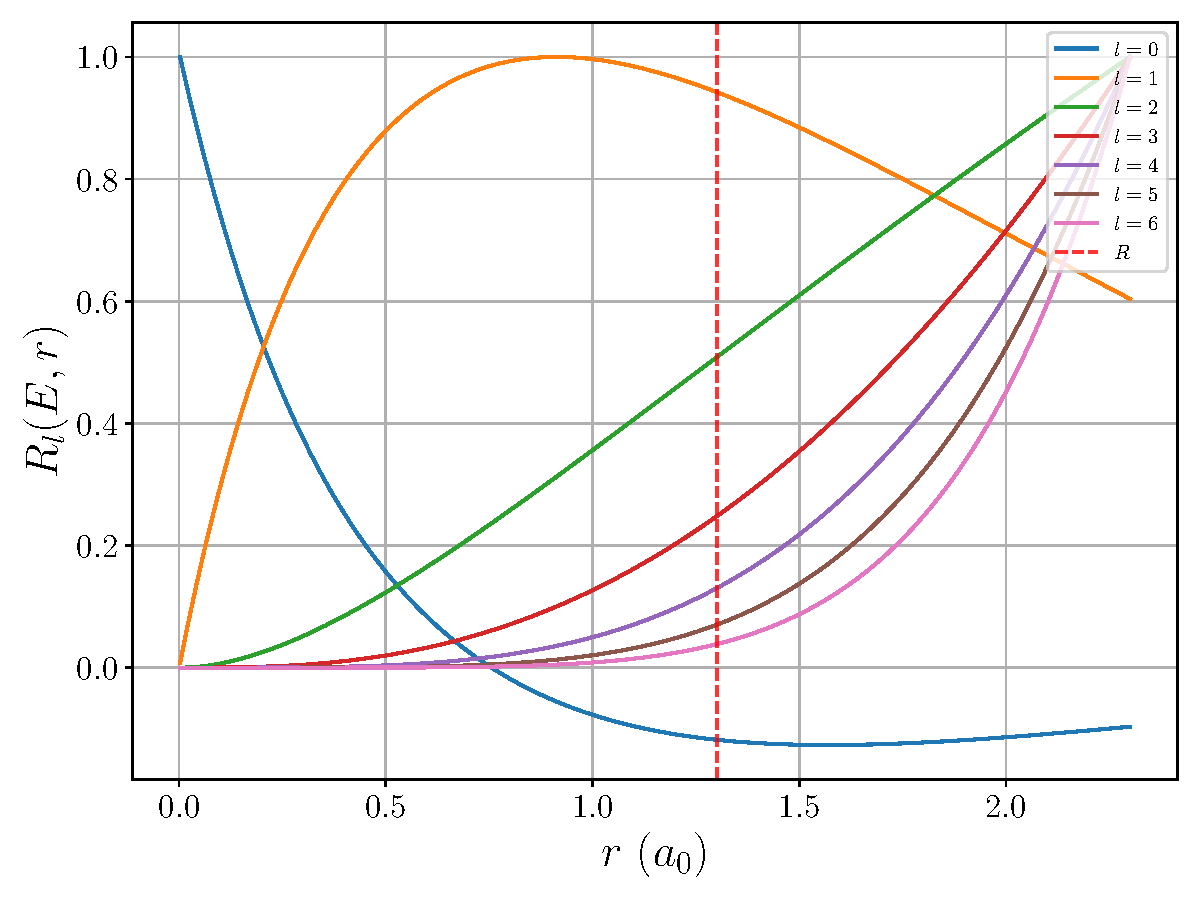
\includegraphics[width=\textwidth]{../plots/mtins/-0.1.pdf}
        \caption{$E = -0.1 \, \text{Ha}$}\
        \label{subfig:mtin_-0.1}
    \end{subfigure}
    \begin{subfigure}{0.49\textwidth}
        \centering 
        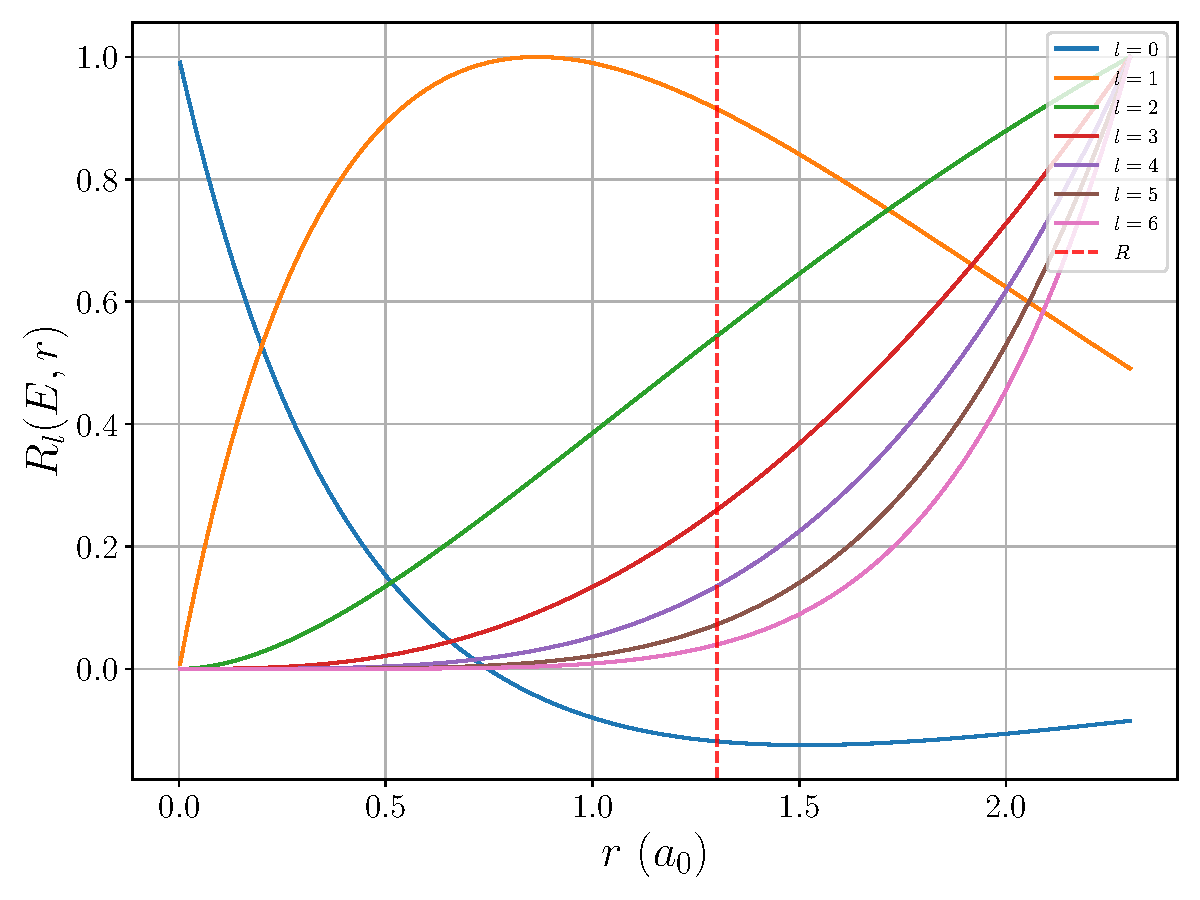
\includegraphics[width=\textwidth]{../plots/mtins/0.pdf}
        \caption{$E = 0.0 \, \text{Ha}$}\
        \label{subfig:mtin_0}
    \end{subfigure}
    \begin{subfigure}{0.49\textwidth}
        \centering 
        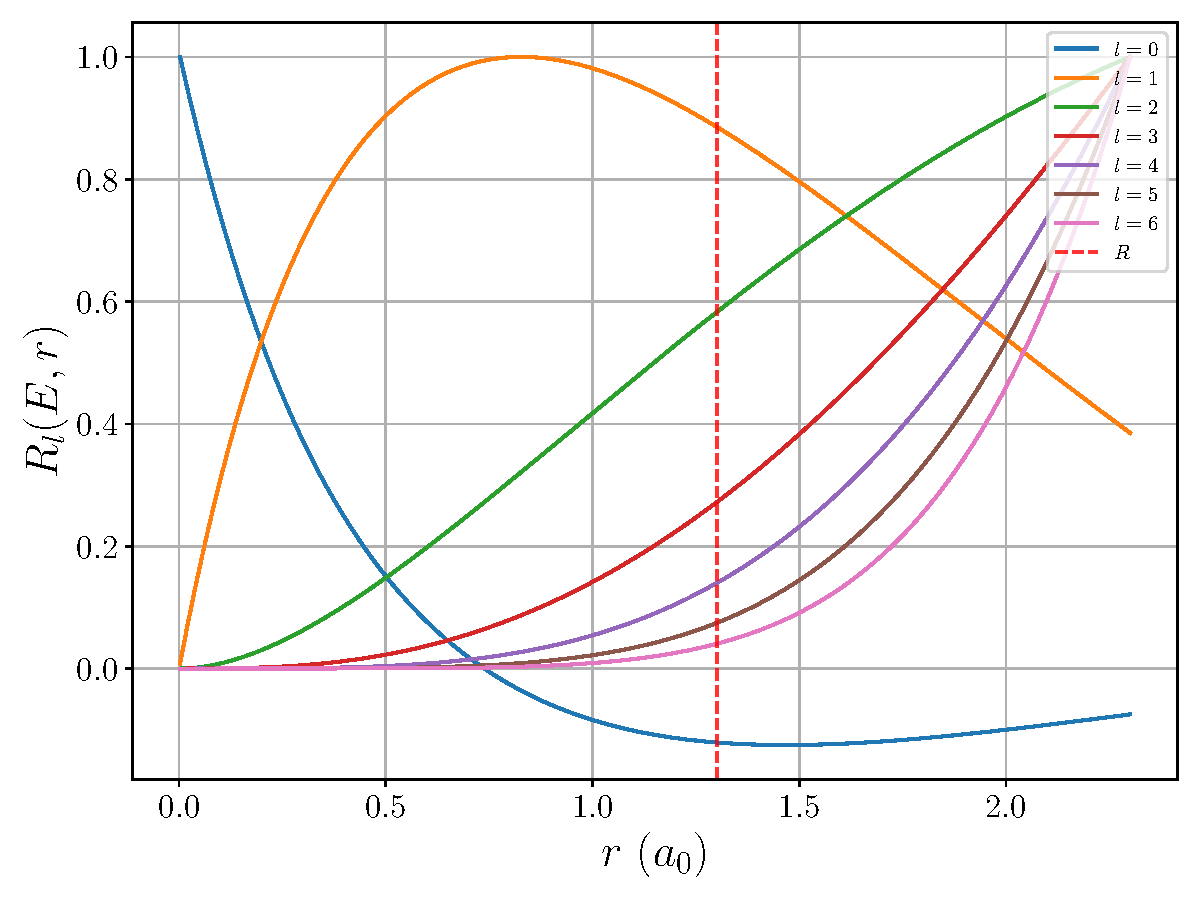
\includegraphics[width=\textwidth]{../plots/mtins/0.1.pdf}
        \caption{$E = 0.1 \, \text{Ha}$}\
        \label{subfig:mtin_0.1}
    \end{subfigure}
    \begin{subfigure}{0.49\textwidth}
        \centering 
        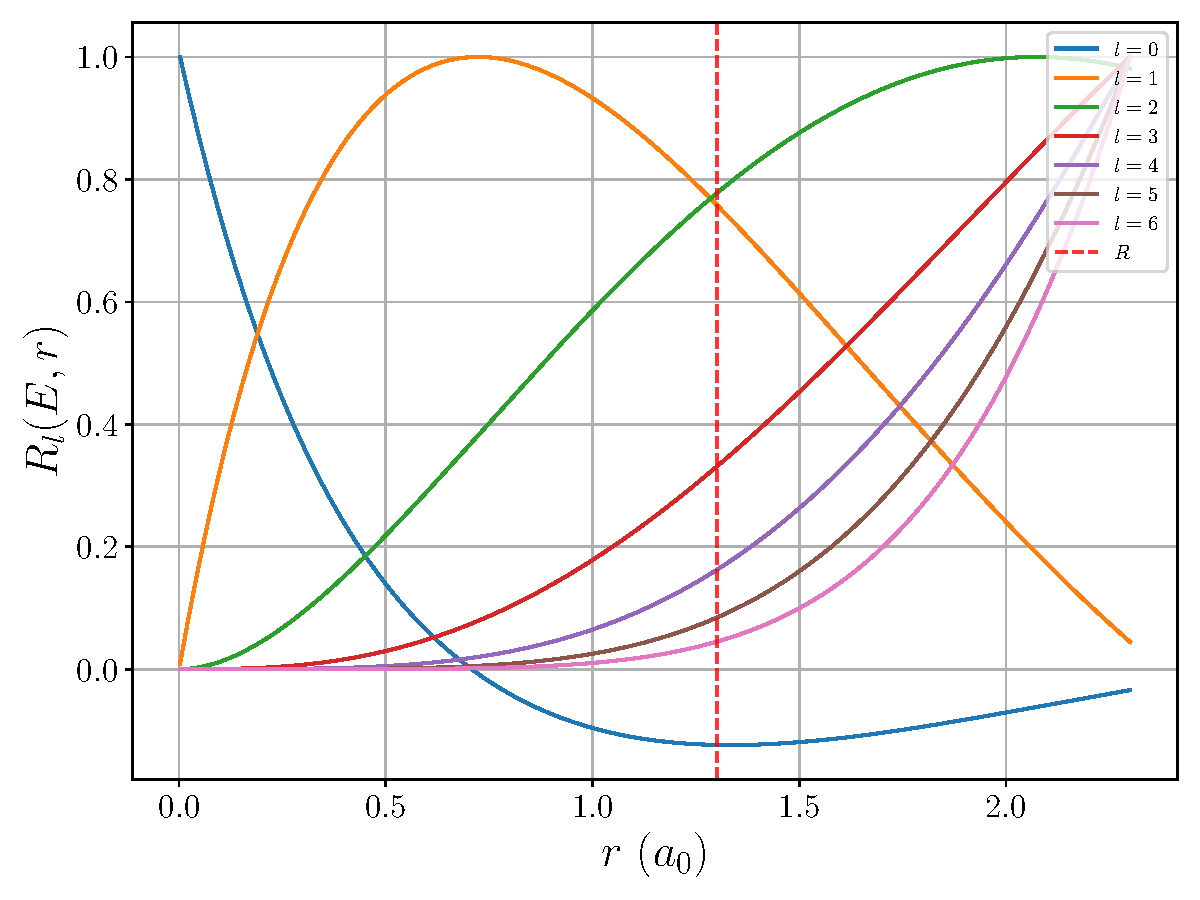
\includegraphics[width=\textwidth]{../plots/mtins/0.5.pdf}
        \caption{$E = 0.5 \, \text{Ha}$}\
        \label{subfig:mtin_-0.5}
    \end{subfigure}
    \caption{Muffin tin functions $E_{l,E}(r)$ for different energies $E$. The muffin tin cut-off radius $R$ is indicated with a vertical line. The functions are artificially scaled to have a maximum value of unity on $[0, 3\,a_0]$, this does not affect the results because only ratios of muffin tin functions and their derivatives appear in the matrix elements of $H_E$.}
    \label{fig:mtins}
\end{figure}

\FloatBarrier
\subsection{Determinants}
\begin{figure}
    \centering 
    \begin{subfigure}{0.49\textwidth}
        \centering 
        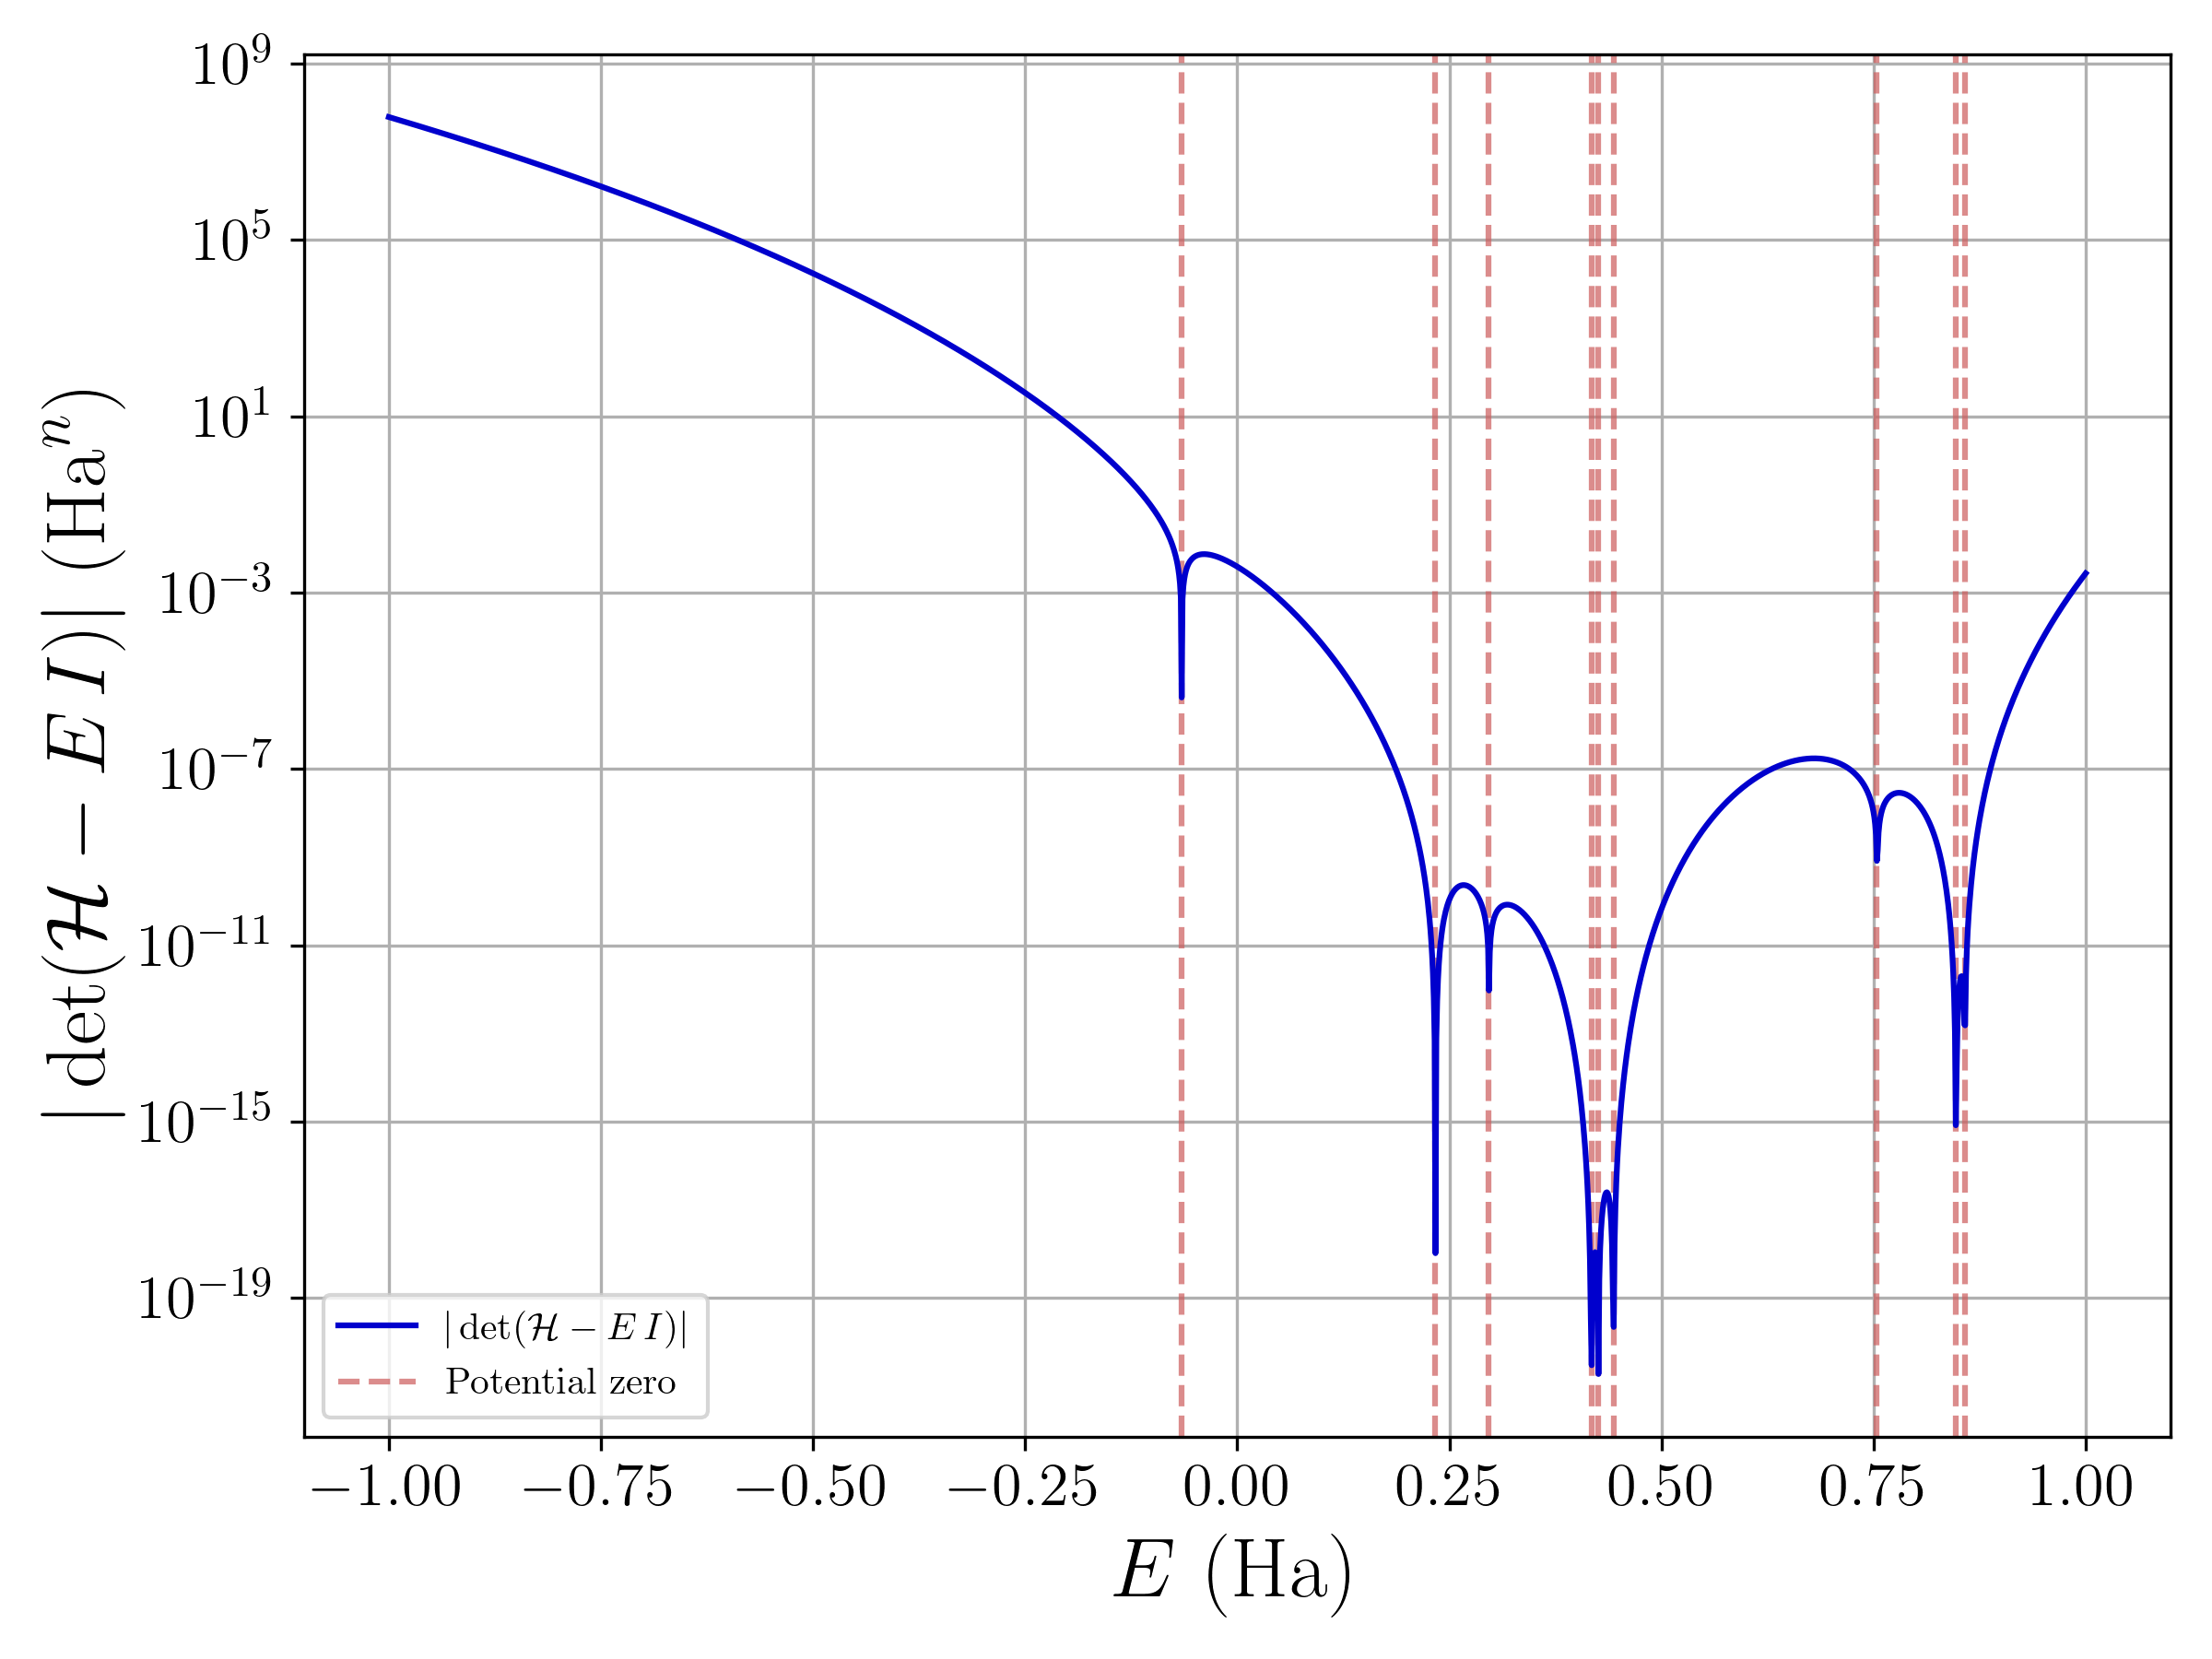
\includegraphics[width=\textwidth]{../plots/det_g_h/det_k_0.0.png}
        \caption{$\textbf{k} = 0$}
        \label{subfig:det0}
    \end{subfigure}
    \begin{subfigure}{0.49\textwidth}
        \centering 
        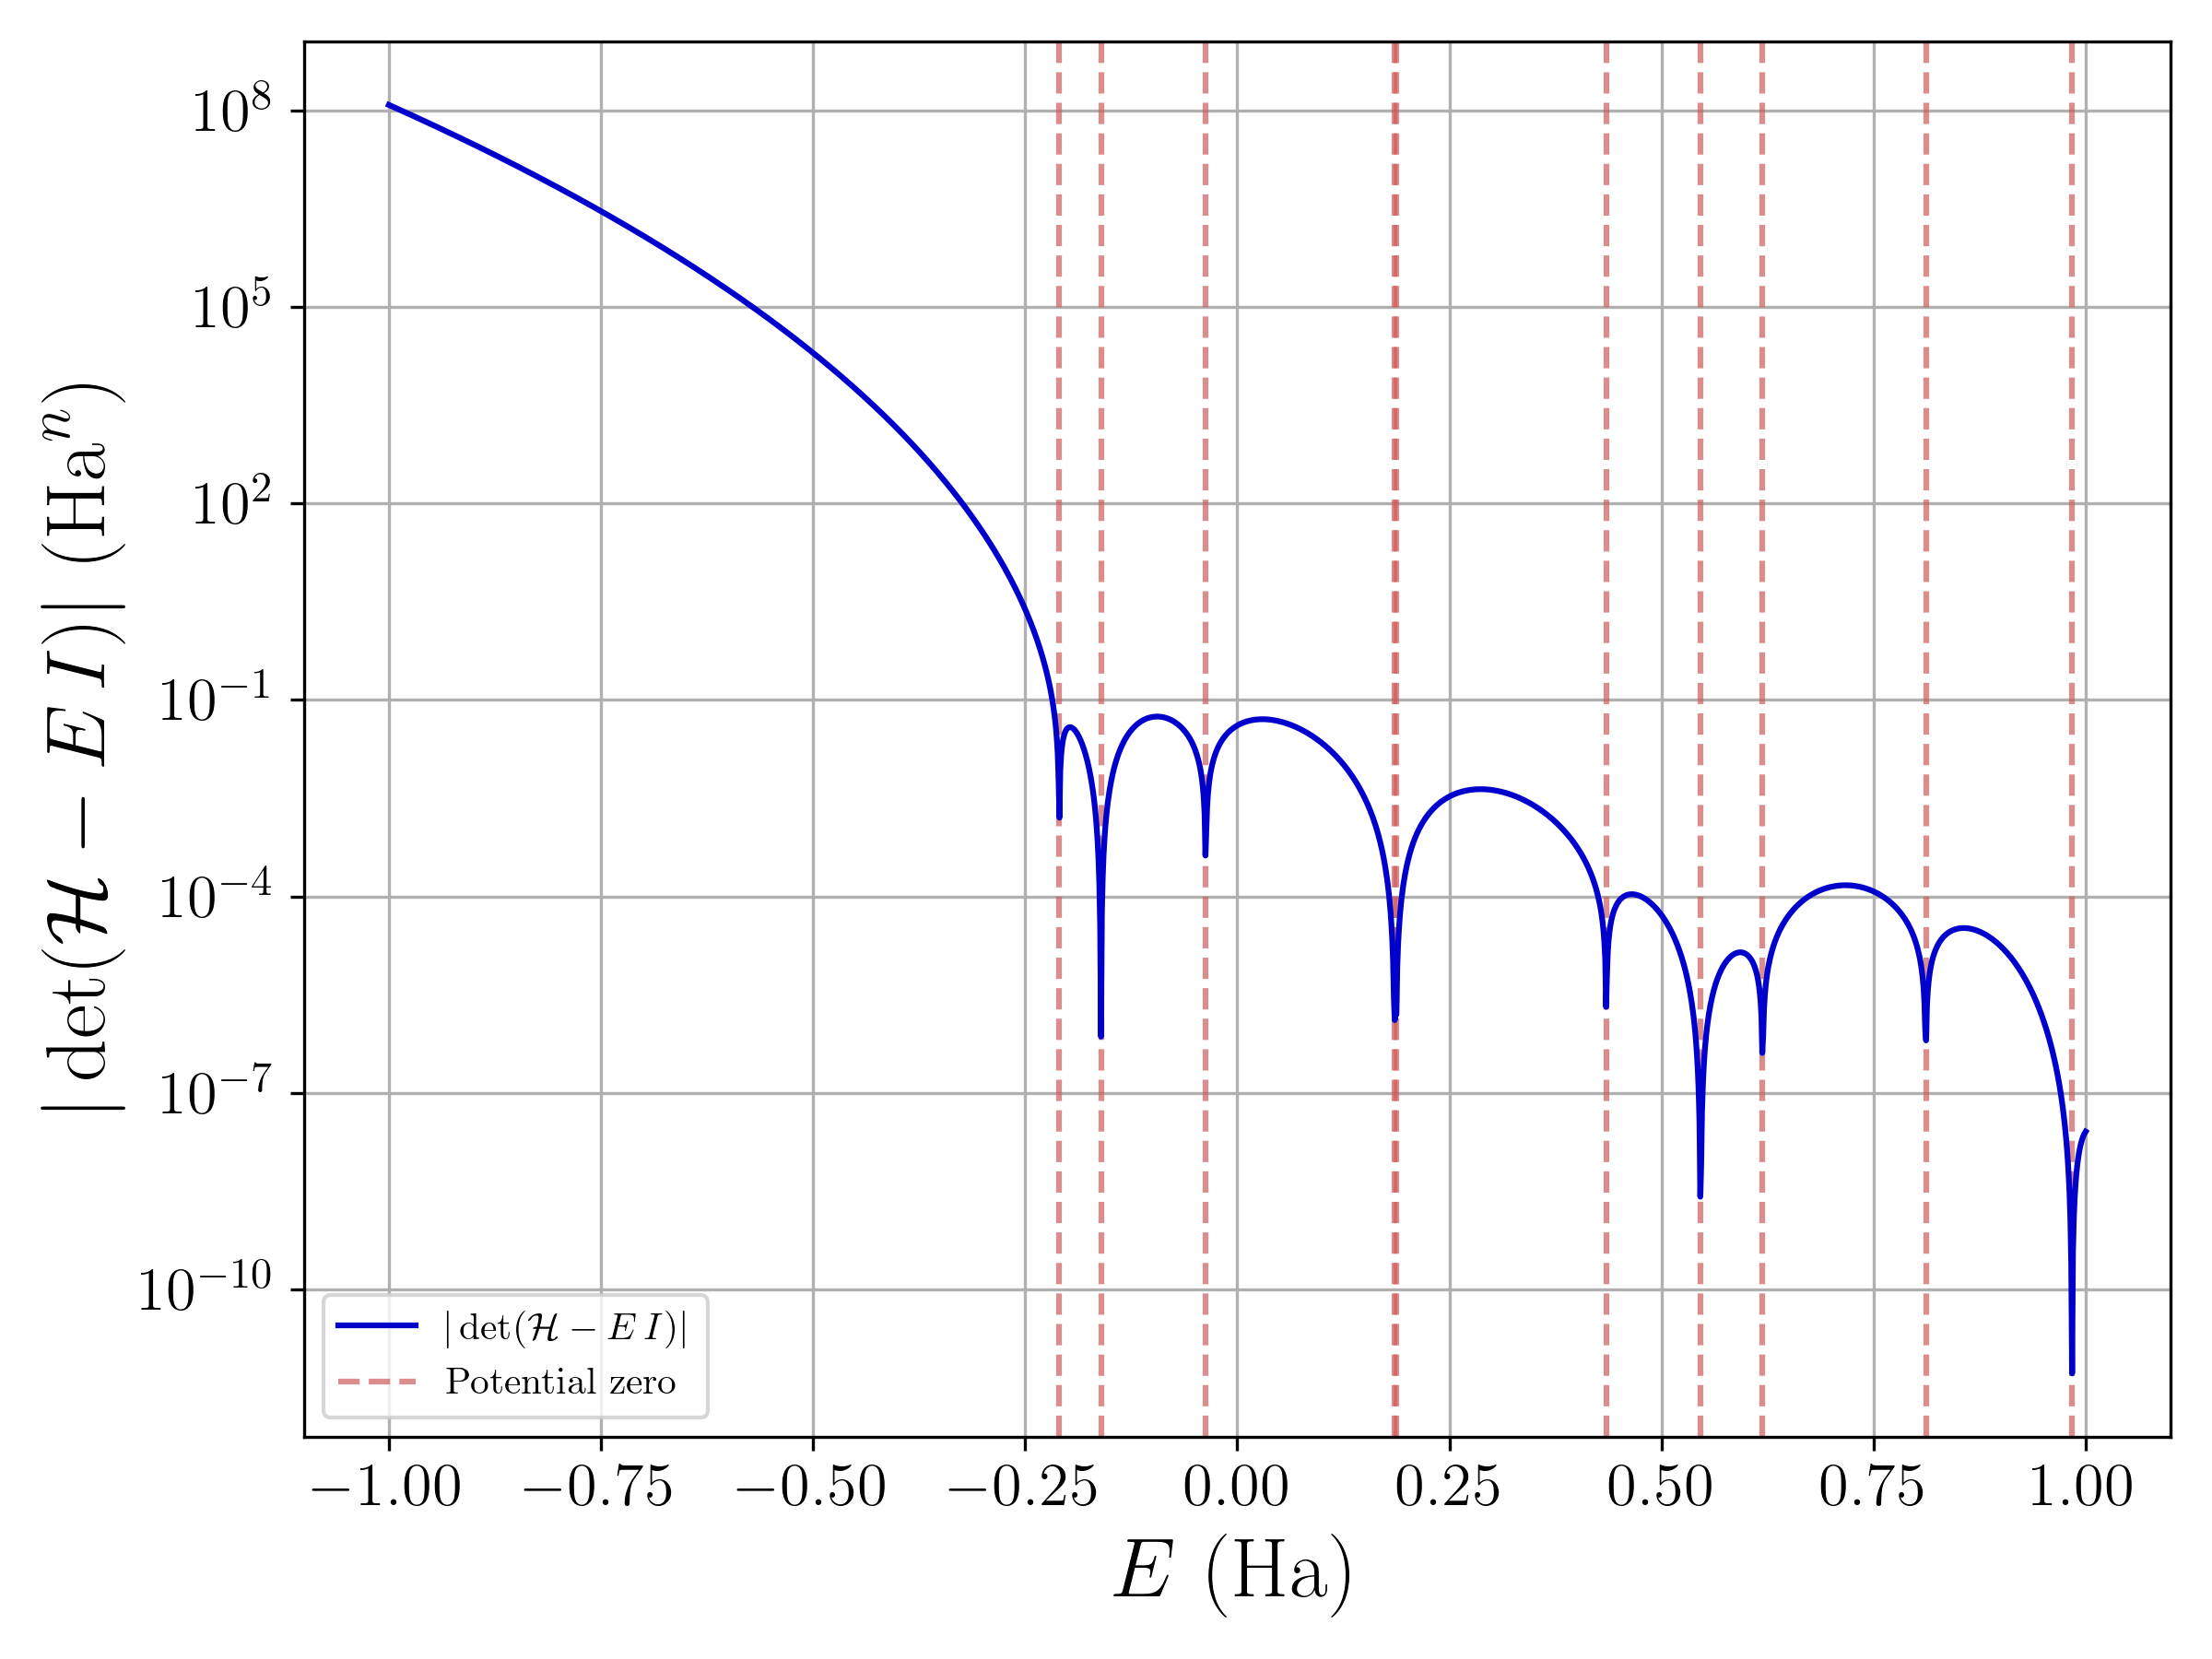
\includegraphics[width=\textwidth]{../plots/det_g_h/det_k_1.0.png}
        \caption{$\textbf{k} = \Gamma$}
        \label{subfig:detG}
    \end{subfigure}
    \caption{Logarithmic absolute value of $\det(H_E - EI)$ for $K_\text{max} = 2/a_0$ and $R=2\,a_0$ at the centre of the BZ~\ref{subfig:det0} and at the Gamma point~\ref{subfig:detG}. Zeros are detected by finding the local minima in the absolute value and are indicated by vertical lines.}
    \label{fig:det}
\end{figure}
To find the electronic spectrum, we have to find the zeros of the determinant $\det(H_E - EI)$. The absolute value of this quantity is shown for two special points in the BZ in figure~\ref{fig:det}. Our chosen approach to find the zeros is to find the relative minima in the determinant. This is not generally guaranteed to work as the function might show local minima, but this is never observed in practice and the bands we get using this method look fine. It is not possible to find the zeros by looking for changes in sign because some roots are higher order.

Note that the value of $R$ used to produce figure~\ref{fig:det} was not used in the rest of the analysis, but there was no time left to reproduce the data needed to make these graphs with a more sensible value of R. We have no reason to expect the qualitative picture to change, though.

\FloatBarrier
\subsection{Band structure}
To find a sensible value of $R$, which is one of the remaining parameter of the model that we have not yet fixed, we employ a pragmatic approach that is though lacking in rigour. We plot the band structure for different $R$ in figure~\ref{fig:bs_var_R}. From literature such as~\cite{perdew_li}, we know that the low bands should touch at the $H$-point. We thus chose $R=1.3$, though $R=1.25$ would also have been a sensible choice.

Having fixed $R$, we can study the influence of the reciprocal lattice sum truncation, i.e.\ the cut-off $K_\text{max}$. It can clearly be seen in figure~\ref{fig:bs} that including more vectors lowers the high-lying bands and alters their shape somewhat. The physics at very low energies is not affected strongly, though, which is in line with expectation. The location of the global energy minimum is unchanged by increasing $K_\text{max}$.

The observation of convergence by going to higher $K_\text{max}$ is supported by figure~\ref{fig:conv}, which shows the deviation of the band structure minimum branch for different $K_\text{max}$. The fact that the deviation is lower everywhere for $3/a_0$ than for $2/a_0$ indicates convergence, though it is hard to say to what error the $K_\text{max} = 4/a_0$ bands have converged. Near the minimum around the $\Gamma$-point, the deviation goes to zero, though, indicating that these points have converged to within the resolution of our energy grid, which as a spacing of $1/1000$ eV.

The value of the Fermi energy included in the band structure plots is read off of a plot in reference~\cite{perdew_li} and as such is not known to high accuracy. Nonetheless, it can clearly be seen that the spectrum of Lithium is gapless and that it is a metal.

The band structure from~\cite{perdew_li} is shown in~\ref{subfig:bs_perdew} and generally shows a very similar scale and similar features as ours, though some details are slightly different, which may be due to the different methods used. We also present a free-electron calculation in~\ref{subfig:bs_free} which shows how some of the coarse structure of the band structure is determined simply by the lattice structure, while the finer structure can only be captured by including more physical effects.

While comparing our results to literature, we noticed they were off by a factor of two. We were not able to identify the source of this problem but have consequently re-scaled all our results presented in this section to fit with literature.

\begin{figure}
    \centering 
    \begin{subfigure}{0.49\textwidth}
        \centering 
        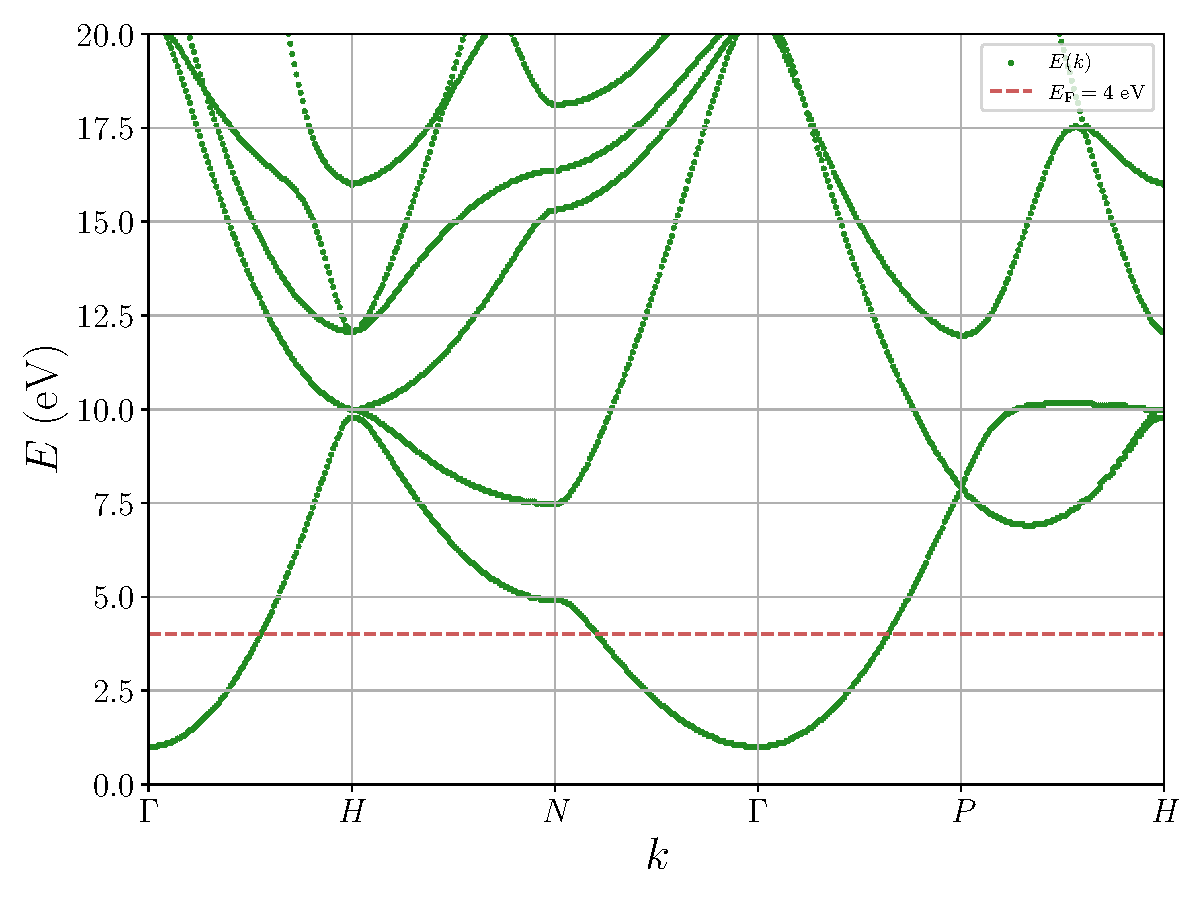
\includegraphics[width=\textwidth]{../plots/bs_2_R_125.pdf}
        \caption{$R=1.25\,a_0$}
        \label{subfig:bs_2_125}
    \end{subfigure}
    \begin{subfigure}{0.49\textwidth}
        \centering 
        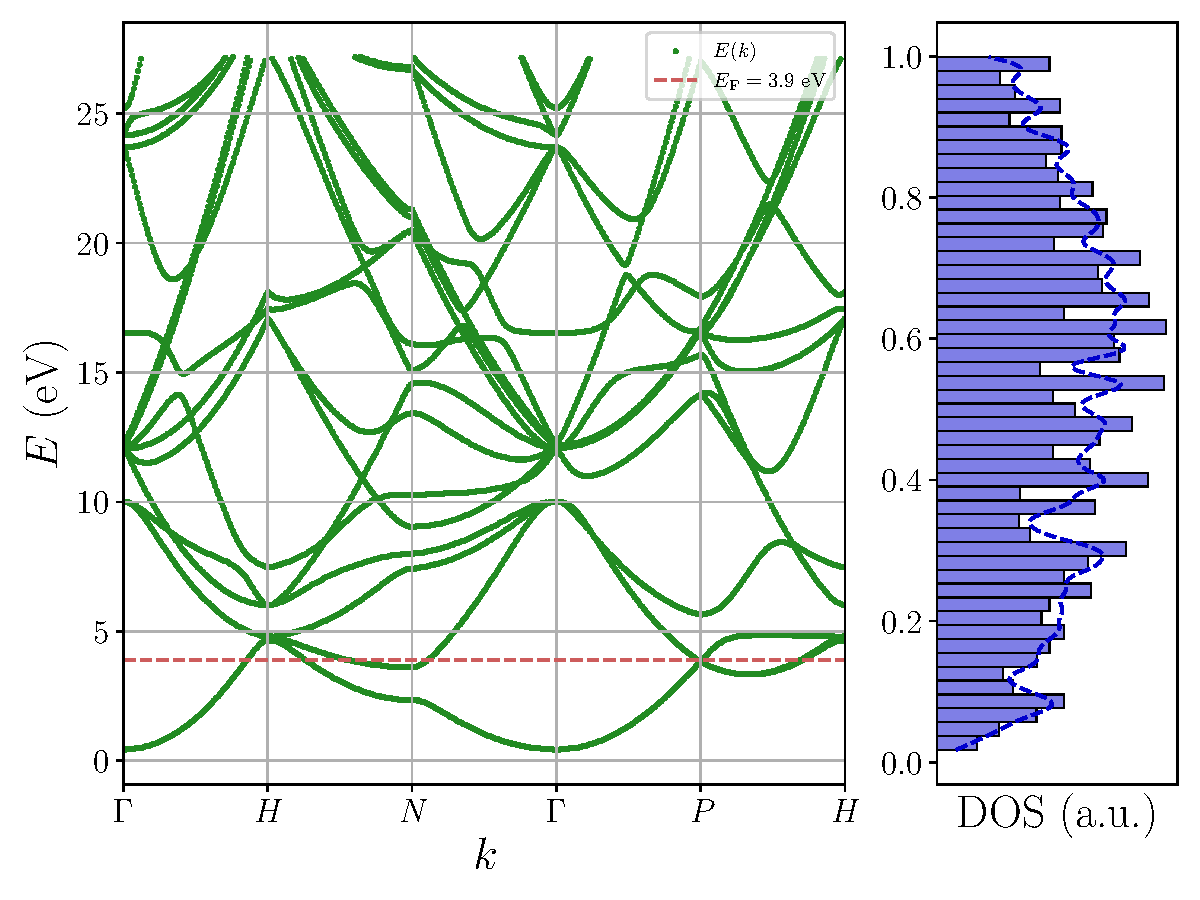
\includegraphics[width=\textwidth]{../plots/bs_2_R_130.pdf}
        \caption{$R=1.30\,a_0$}
        \label{subfig:bs_2_130}
    \end{subfigure}
    \begin{subfigure}{0.49\textwidth}
        \centering 
        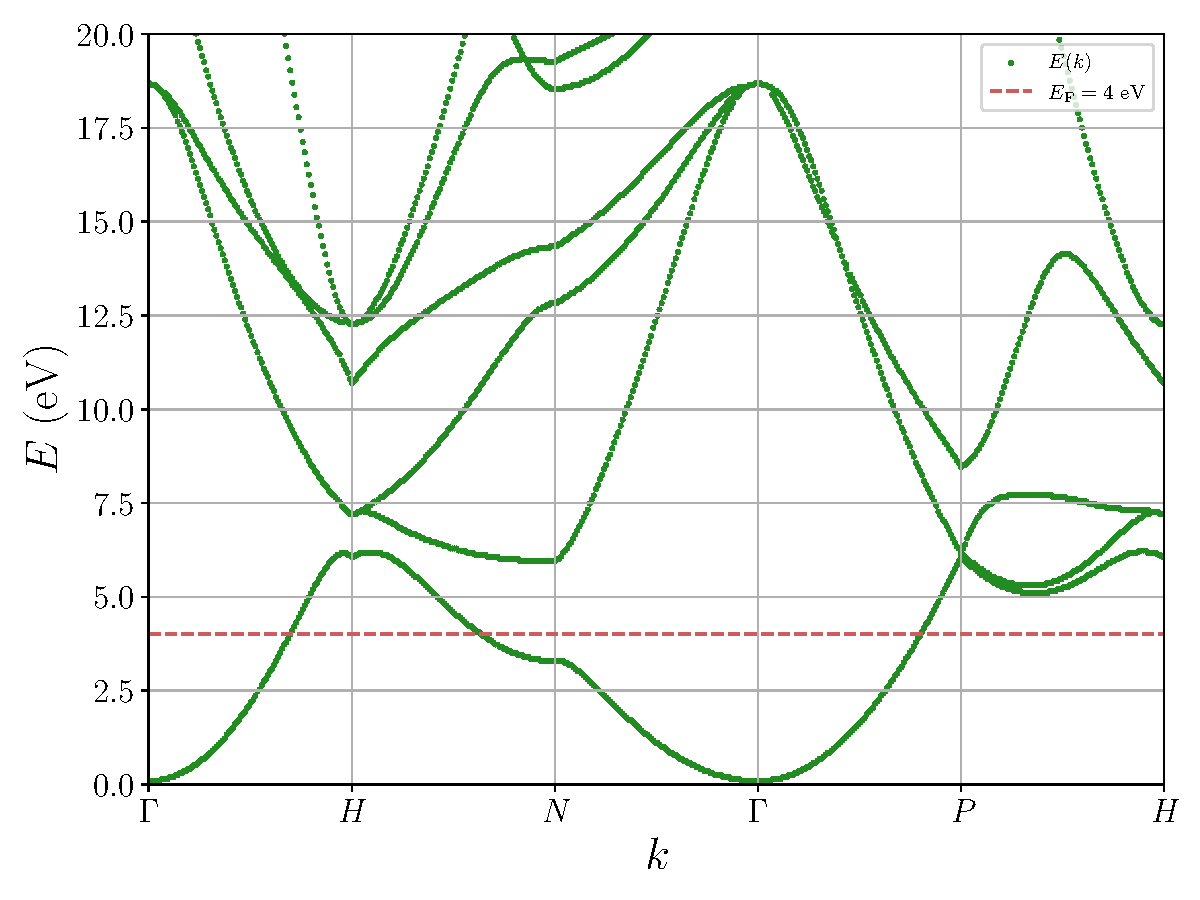
\includegraphics[width=\textwidth]{../plots/bs_2_R_150.pdf}
        \caption{$R=1.50\,a_0$}
        \label{subfig:bs_2_150}
    \end{subfigure}
    \caption{Low-accuracy $K_\text{max} = 2/a_0$ bands for different $R$. It is known that the low-lying bands should touch at the $H$-point from literature, e.g.~\cite{perdew_li}, so this should be reproduced by a good choice of $R$.}
    \label{fig:bs_var_R}
\end{figure}

\begin{figure}
    \centering 
    \begin{subfigure}{0.49\textwidth}
        \centering 
        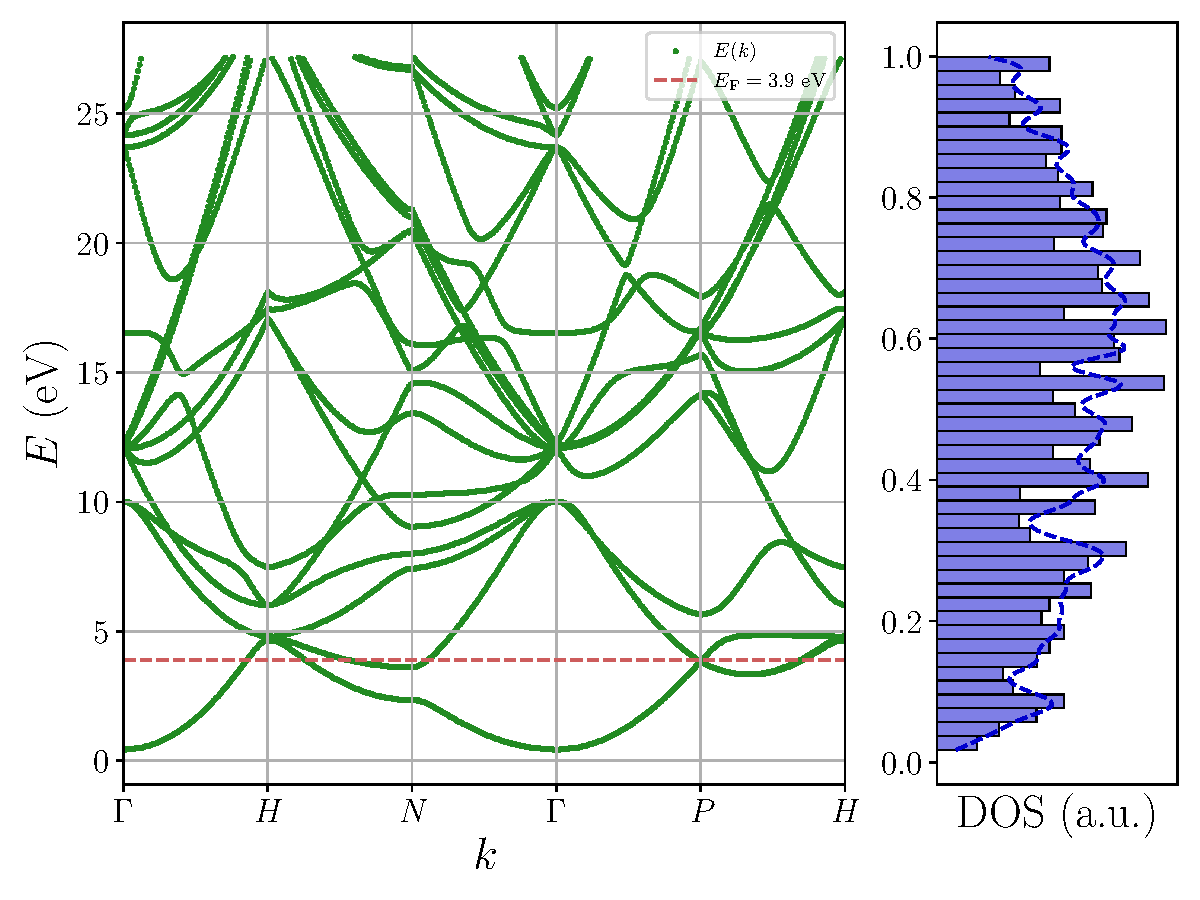
\includegraphics[width=\textwidth]{../plots/bs_2_R_130.pdf}
        \caption{$K_\text{max} = 2/a_0$}
        \label{subfig:bs_2_130_2}
    \end{subfigure}
    \begin{subfigure}{0.49\textwidth}
        \centering 
        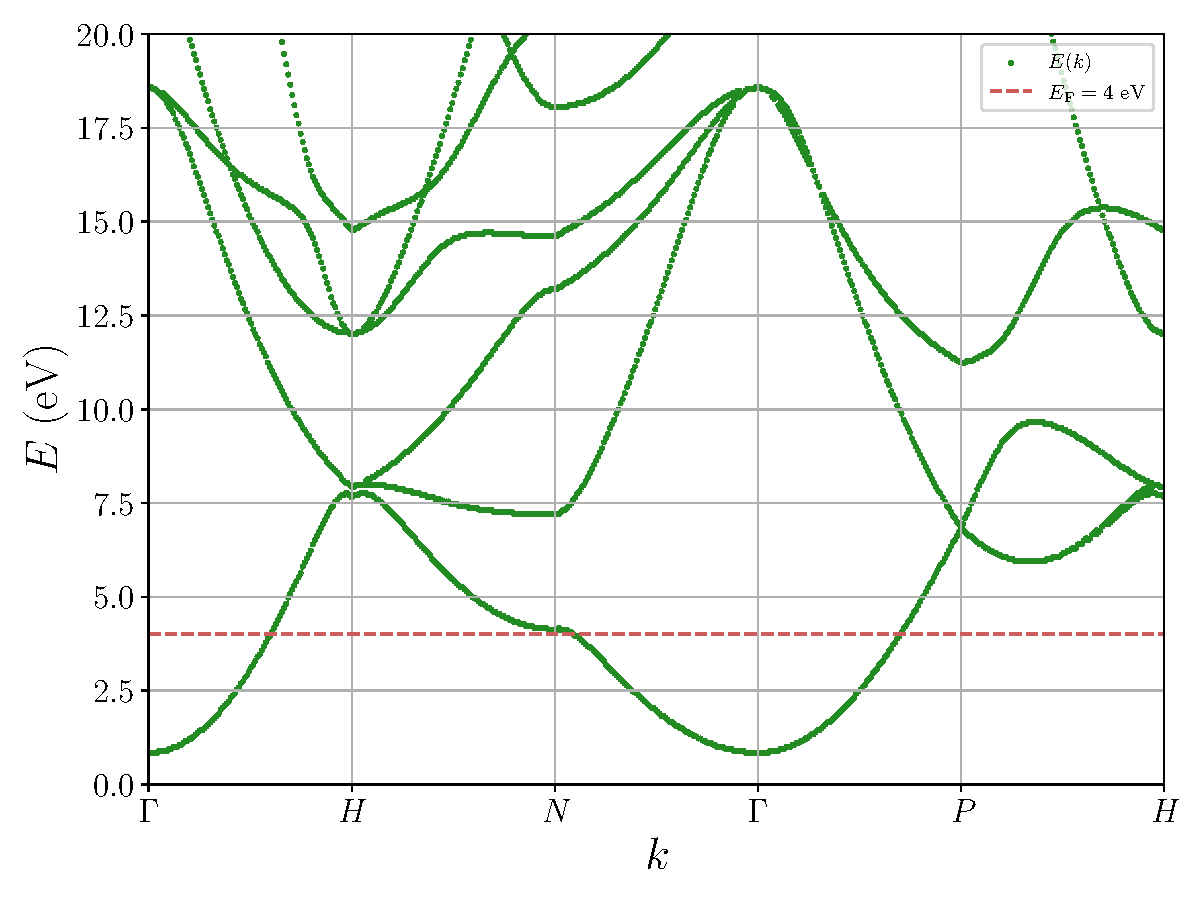
\includegraphics[width=\textwidth]{../plots/bs_3_R_130.pdf}
        \caption{$K_\text{max} = 3/a_0$}
        \label{subfig:bs_3_130}
    \end{subfigure}
    \begin{subfigure}{0.49\textwidth}
        \centering 
        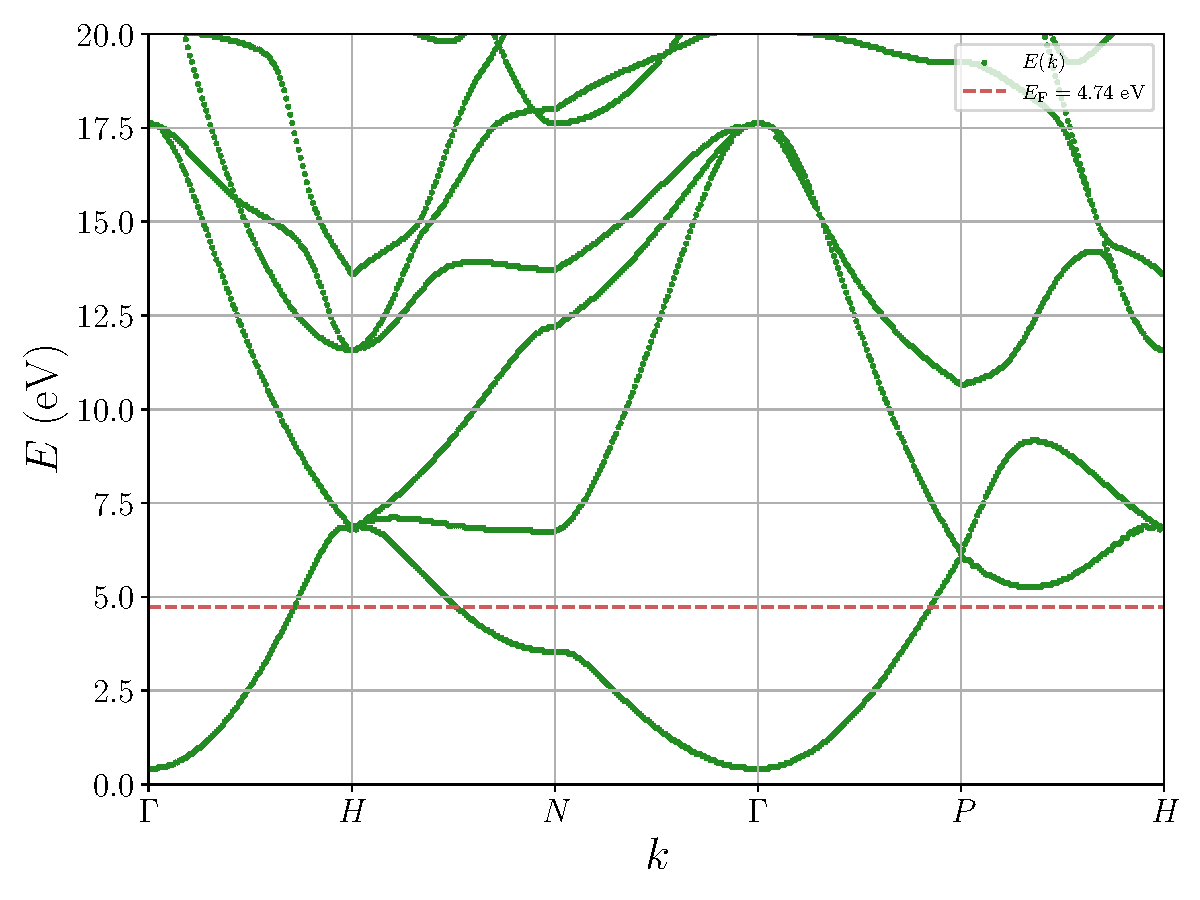
\includegraphics[width=\textwidth]{../plots/bs_4_R_130.pdf}
        \caption{$K_\text{max} = 4/a_0$}
        \label{subfig:bs_4_130}
    \end{subfigure}
    \begin{subfigure}{0.49\textwidth}
        \centering 
        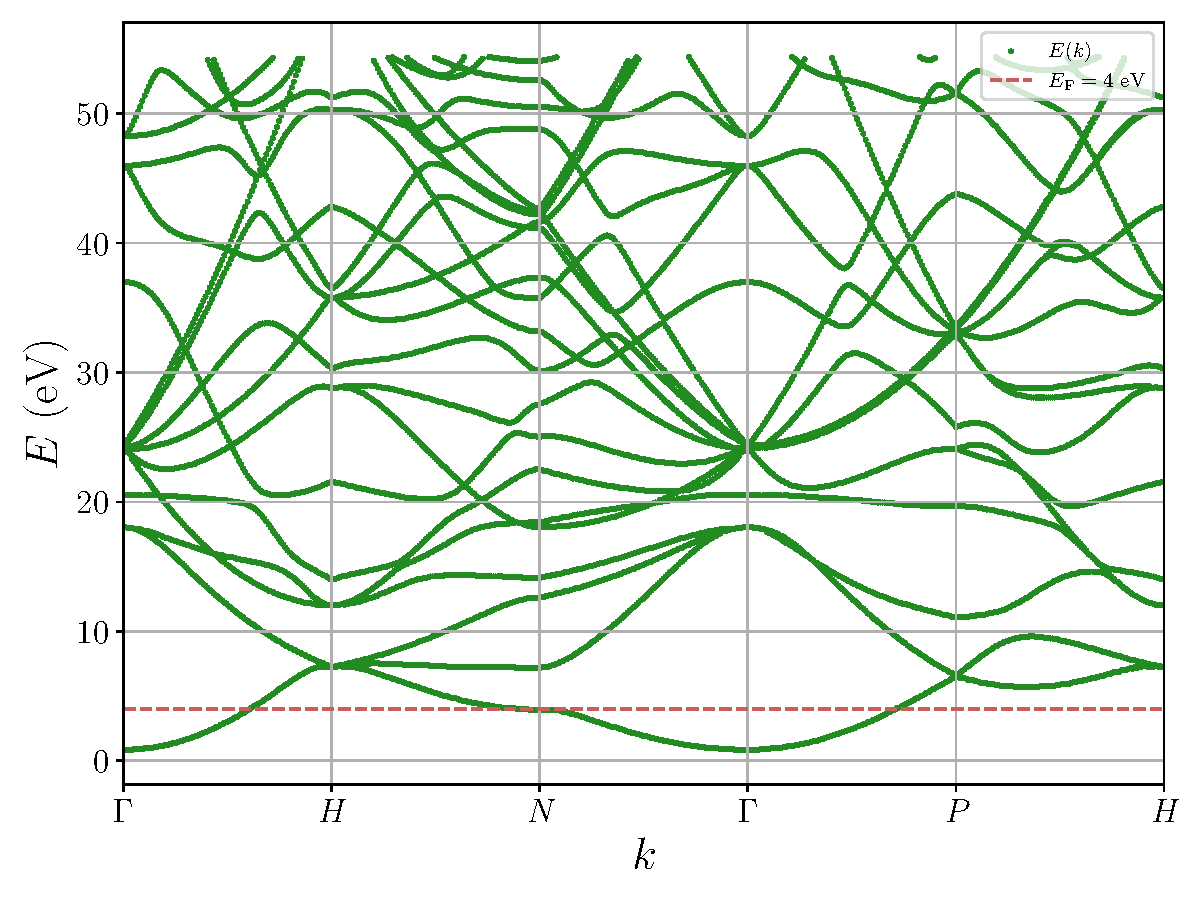
\includegraphics[width=\textwidth]{../plots/bs_4_R_130_full.pdf}
        \caption{$K_\text{max} = 4/a_0$, full range}
        \label{subfig:bs_4_130_full}
    \end{subfigure}
    \begin{subfigure}{0.49\textwidth}
        \centering 
        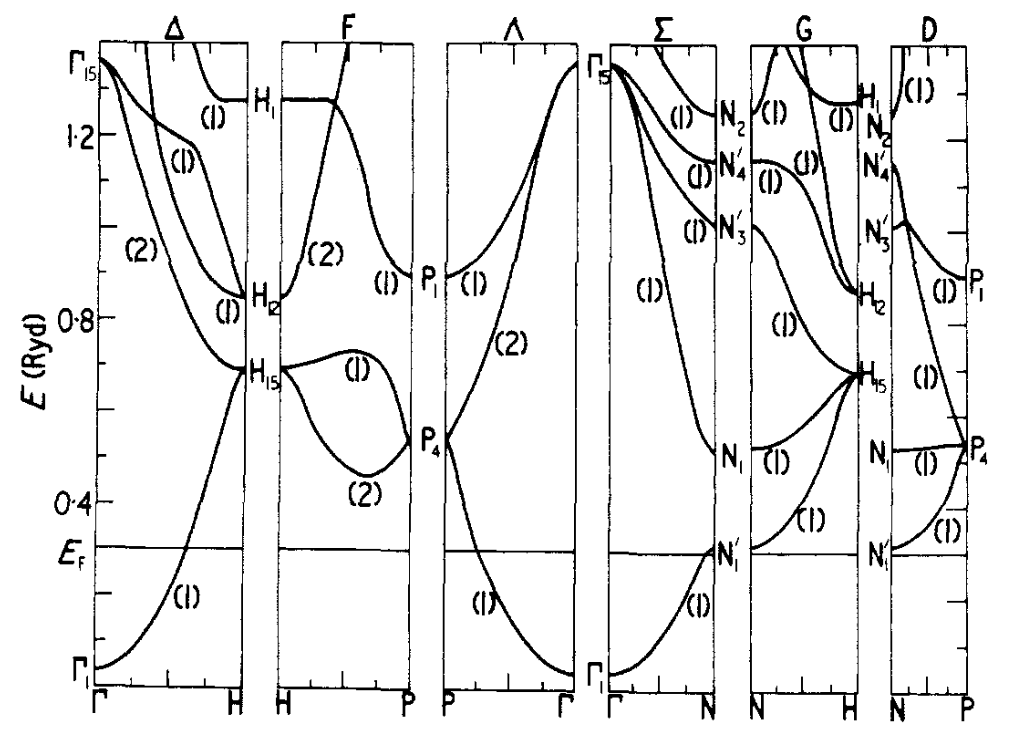
\includegraphics[width=\textwidth]{./fig/bs.png}
        \caption{Calculation from~\cite{perdew_li}}
        \label{subfig:bs_perdew}
    \end{subfigure}
    \begin{subfigure}{0.49\textwidth}
        \centering 
        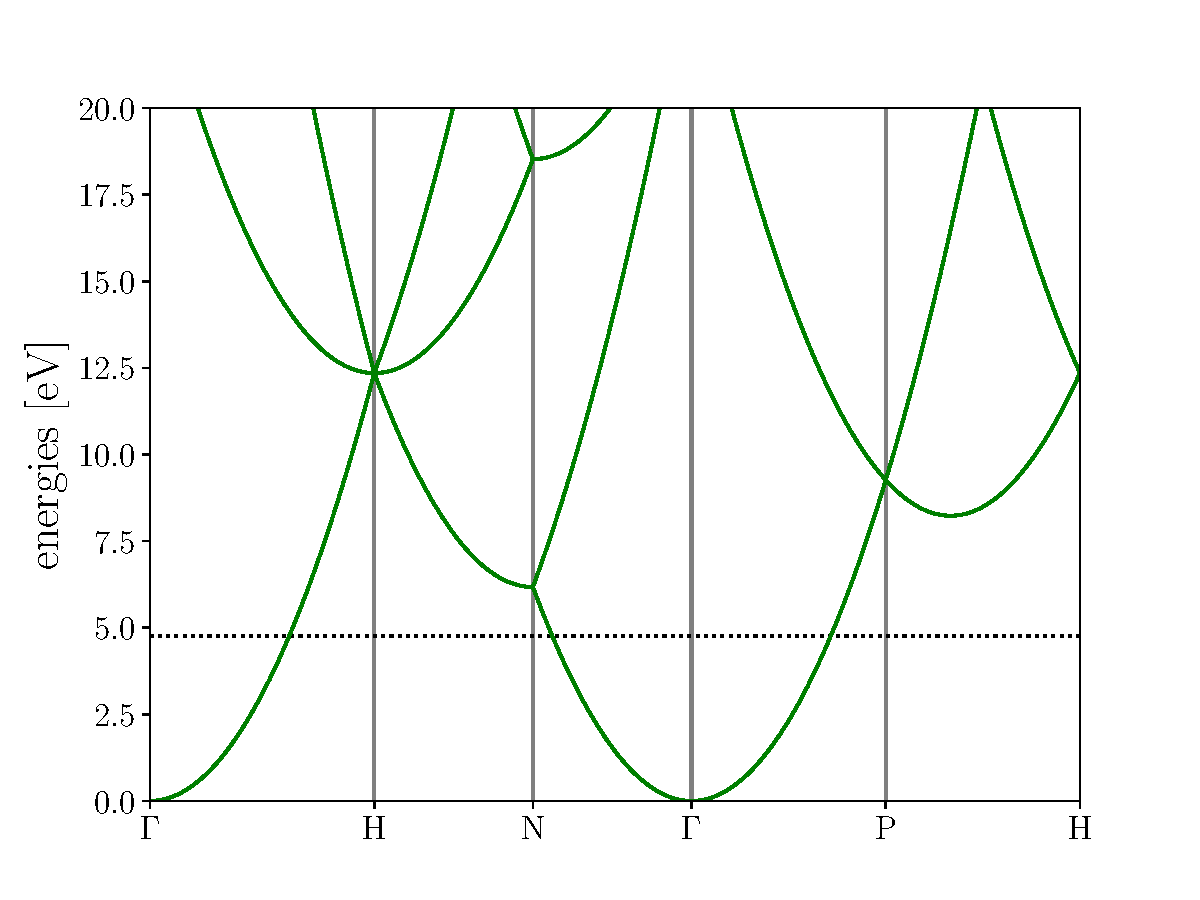
\includegraphics[width=\textwidth]{../src/py/li.pdf}
        \caption{Free electrons using~\cite{ase-paper}}
        \label{subfig:bs_free}
    \end{subfigure}
    \caption{Lithium band structure using APWs (\ref{sub@subfig:bs_2_130_2} - \ref{subfig:bs_4_130_full}), orthogonalised plane waves~\cite{perdew_li} and for free electrons calculated using the ASE package~\cite{ase-paper}. It can be seen for the APW plots that including more reciprocal lattice vectors seemingly leads to a convergence in the band structure. Comparing the APW band structure to the free electrons, some similar large scale structures can be observed, but the free electron bands are quadratic while the APW bands are more complicated. The OPW calculation shows similar features, both quantitatively and qualitatively. $E_\text{F}$ in APW plots from~\cite{perdew_li}.}
    \label{fig:bs}
\end{figure}

\begin{figure}
    \centering 
    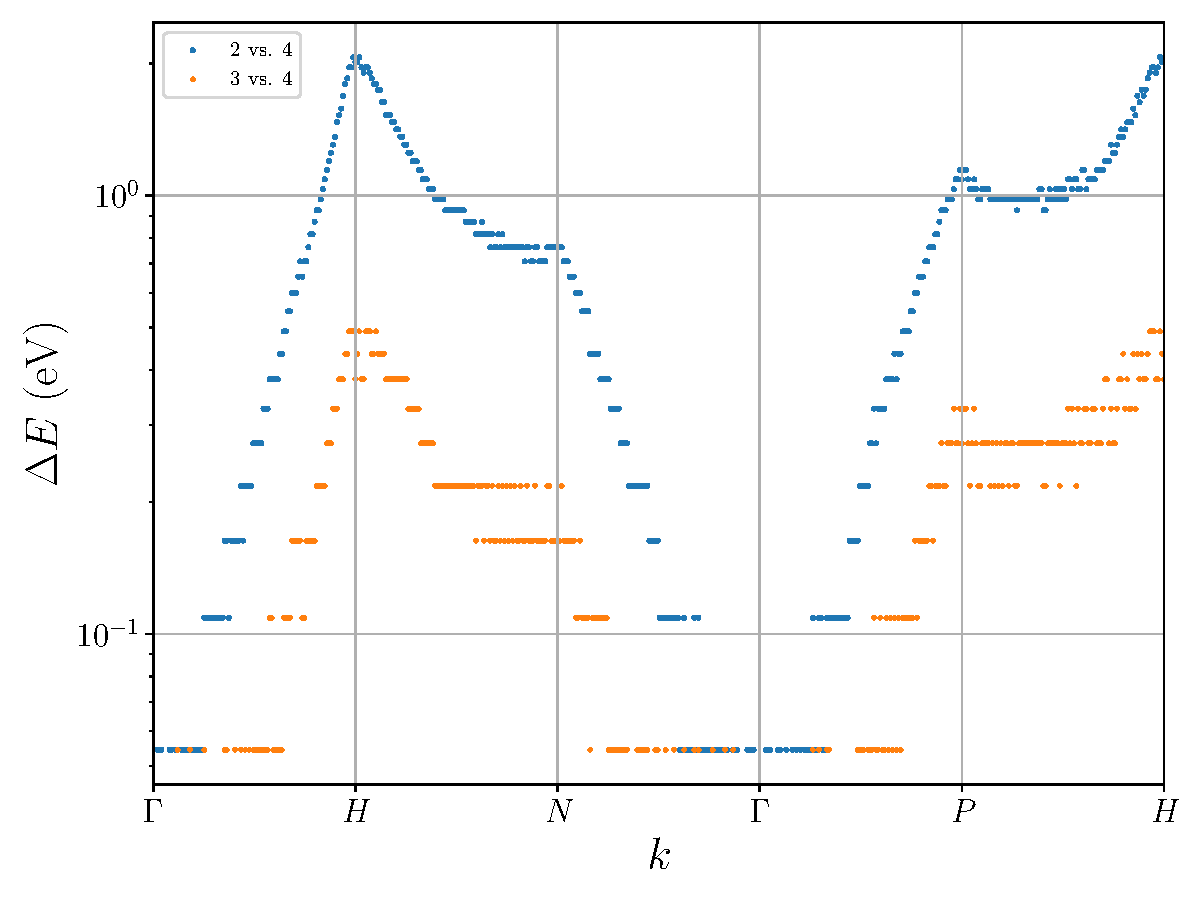
\includegraphics[width=0.65\textwidth]{../plots/conv_24.pdf}
    \caption{Deviation of the band structure minimum branch for $K_\text{max} = 2/a_0$ vs. $4/a_0$ and $3/a_0$ vs. $4/a_0$, respectively. The fact that the deviation is lower everywhere for $3/a_0$ indicates convergence, though it is hard to say to what error the $K_\text{max} = 4/a_0$ bands have converged.}
    \label{fig:conv}
\end{figure}

\FloatBarrier
\subsection{Density of States}
Finally, it is interesting to see how many available states there are at a given energy. This is indicated by the density of states (DOS)
\begin{equation}
    D(E) = \frac{1}{V} \sum_i \delta(E - E_i) = 2\int_{\mathbb{R}^3} \frac{\text{d}^3k}{(2\pi)^3}\delta(E-E(\textbf{k})),
\end{equation}
where the last equality is only valid if the energy does not depend on spin and $E(\textbf{k})$ is non-degenerate.

To this end, we compute the energies on a grid spanning the entire BZ. This is not the most efficient approach, because the BZ has symmetries which should enable one to restrict the grid to a small wedge, also referred to as an irreducible wedge. We did not attempt this however and accepted the loss in resolution.

Due to the high computational demands, we were only able to finish these calculations for $K_\text{max}=2$. Figure~\ref{fig:bs_2_DOS} shows the band structure and a histogram of the state density. A free electron gas has a DOS that scales as $\sqrt{E}$. We also observe that the DOS is increasing for small $E$, while it is oscillating for higher $E$. Furthermore, it is decreasing towards higher energies. 

\begin{figure}
    \centering
    \begin{subfigure}{0.49\textwidth}
        \centering 
        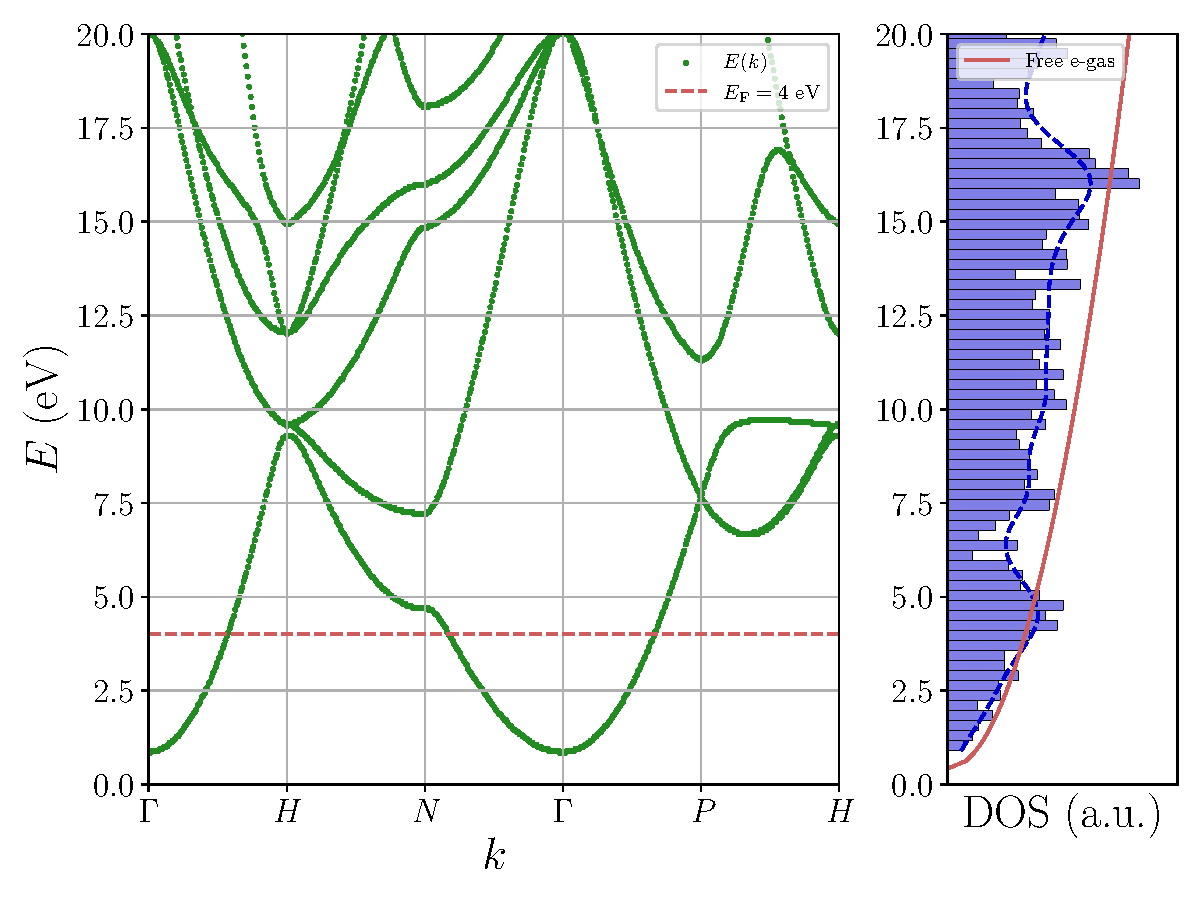
\includegraphics[width=\textwidth]{../plots/bs_2_R_130_DOS.pdf} 
        \caption{Small range}
        \label{subfig:bs_dos_zoom}        
    \end{subfigure}
    \begin{subfigure}{0.49\textwidth}
        \centering 
        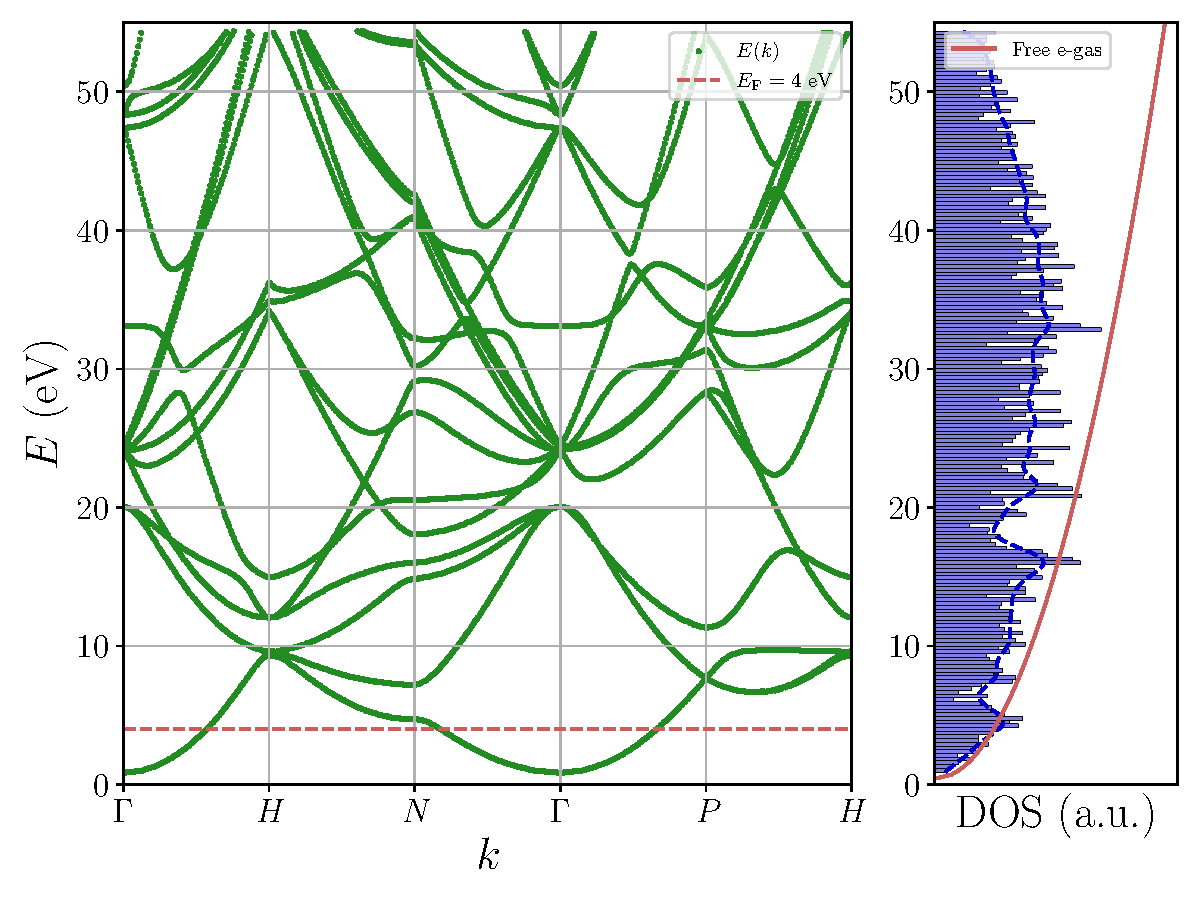
\includegraphics[width=\textwidth]{../plots/bs_2_R_130_full_dos.pdf} 
        \caption{Full range}
        \label{subfig:bs_dos_full}        
    \end{subfigure}
    \caption{$K_\text{max} = 2/a_0$ Li band structure including the binned density of states. Note that the DOS is calculated from points all over the BZ, not just along the paths of high symmetry. Free electron gas DOS $\sim \sqrt{E}$ is indicated in the plot, but has only been scaled to allow for a rough quantitative comparison, not a qualitative one.}
    \label{fig:bs_2_DOS}
\end{figure}

\FloatBarrier
\section{Conclusion}
We have successfully implemented the APW method and applied it to lithium. In principle, it should generate to other elements with moderate effort but in practice we are limited by the atomic DFT calculations not converging for many of the elements beyond Caesium, which is why elements such as Copper could not be treated without modifying some of the underlying codebase.

It would also have been interesting to study the Fermi surface of Lithium and some attempts to this end were made, though they remained unsuccessful and were thus omitted from this report.


\FloatBarrier
\newpage
\fakesection{References}
\printbibliography


\end{document}
